\documentclass[11pt,titlepage]{report}

%%%%%%%%%%%%%%%%%%%%%%%%%%%%%%%%%%%%%%%%%%%%%%%%%%%%%%%%%%%%%%%%%%%%%%%%%%%%%%%
% For new proposals, sections may need to be (un)commented and reordered
% to reflect that requested in FOA
%%%%%%%%%%%%%%%%%%%%%%%%%%%%%%%%%%%%%%%%%%%%%%%%%%%%%%%%%%%%%%%%%%%%%%%%%%%%%%%

%%%%% Setup packages, style, etc. %%%%%%%%%%%%%%%%%%%%%%%%%%%%%%%%%%%%%%%%%%%%%
%%%%%%%%%%%%%%%%%%%%%%%%%%%%%%%%%%%%%%%%%%%%%%%%%%%%%%%%%%%%%%%%%%%%%%%%%%%%%%
% Setup packages, style, additional commands, etc.
% $Id$
%%%%%%%%%%%%%%%%%%%%%%%%%%%%%%%%%%%%%%%%%%%%%%%%%%%%%%%%%%%%%%%%%%%%%%%%%%%%%%%
\newcommand{\zapspace}[0]{}
\usepackage[letterpaper,textheight=9in,textwidth=6.5in,margin=1in]{geometry}

\usepackage[utf8]{inputenc}     % Better for text pasted from Word & such
\usepackage[T1]{fontenc}
\usepackage{bigstrut}           % Used by Excel2LATeX exports
\usepackage{amsmath}            % Used by OpenOffice LaTeX exporter
% packages above (probably amsmath) need to preceed fxfonts
\usepackage{txfonts}            % Use native postscript fonts

\usepackage{cite}
\usepackage{varioref}
\usepackage{url}
\usepackage{color}
%%%\usepackage{svn}
\usepackage{listings}
%%\usepackage[bookmarks=false,pdfpagelayout=SinglePage]{hyperref}
\usepackage[bookmarksopen=true,bookmarksopenlevel=0,pdfpagelayout=SinglePage]{hyperref}

\usepackage{longtable}
% Default caption width for longtable environments
\setlength{\LTcapwidth}{\textwidth}
\usepackage{multirow}
\usepackage[font=it,labelfont=bf]{caption}
\usepackage{sidecap}            % Alternative to constructing minipages
\usepackage{tabularx}
\usepackage{ragged2e}
\usepackage{rotating}

\usepackage{fancyhdr}
\usepackage{graphicx} 
\usepackage{caption}
\usepackage{wrapfig}
\usepackage{pdfpages}
\usepackage[compact]{titlesec}
%%% \usepackage[iso]{datetime}
%%% \settimeformat{ampmtime}        % Override iso time format
%%%\usepackage{xcomment}
%%%\usepackage{paralist}           % Provides compact versions of lists
\usepackage{enumitem}
\usepackage{ifthen}
\usepackage{rotating}
\usepackage{listings}
\usepackage{calc}                  % Used in participant table construction

\usepackage{minitoc}            % Load after caption (if used)
\usepackage{etoolbox}

%%%%% Packages to avoid, and alternatives
% epsfig: already using graphicx
% here: use [!ht] or float.sty [H] instead
% times: txfonts

% remove red border around links (comment out if you want the border)
%\hypersetup{pdfborder={0 0 0}}

%%%%% Control what is processed %%%%%%%%%%%%%%%%%%%%%%%%%%%%%%%%%%%%%%%%%%%%%%%
% Requires ifthen package loaded

%%%%%%%%%%%%%%%%%%%%%%%%%%%%%%%%%%%%%%%%%%%%%%%%%%%%%%%%%%%%%%%%%%%%%%%%%%%%%%%
% Define what will be included in the document
%%%%%%%%%%%%%%%%%%%%%%%%%%%%%%%%%%%%%%%%%%%%%%%%%%%%%%%%%%%%%%%%%%%%%%%%%%%%%%%
% Shorthand for providing and initially setting
\newcommand{\provBoolDflt}[2]{
   \provideboolean{#1}
   \setboolean{#1}{#2}
}

% There ought to be a simpler way, but I couldn't find in Google
% First argument is set to result of logical AND of first and second
\newcommand{\booleanand}[2]{
  \ifthenelse{\boolean{#1} \and \boolean{#2} }{
    \setboolean{#1}{true}
  }{
    \setboolean{#1}{false}
  }
}

% For debugging
\newcommand{\typeoutboolean}[2]{
  \ifthenelse{\boolean{#2}}{
    \typeout{#1 #2 = TRUE}
  }{
    \typeout{#1 #2 = FALSE}
  }
}

%%%%% Read in user configuration %%%%%%%%%%%%%%%%%%%%%%%%%%%%%%%%%%%%%%%%%%%%%%
%%%%%
%%%%% Set defaults, then read in user's configuration file (if one
%%%%% exists) to override them.

\newcommand{\proposalinstitution}{ornl} %%% One of the participating insts
\newcommand{\proposallead}{ornl}      %%% institution leading the proposal
\newcommand{\proposalcontent}{lab}  %%% technical|lab|grants|abstract|public
\newcommand{\proposalversion}{draft} %%% draft|final

\IfFileExists{configure.tex}{
   % Generated by Makefile Sat May 23 17:17:44 EDT 2015
\renewcommand{\proposallead}{ornl}
\renewcommand{\proposalinstitution}{ornl}
\renewcommand{\proposalcontent}{lab}

}{}

%%%%% Available/required content %%%%%%%%%%%%%%%%%%%%%%%%%%%%%%%%%%%%%%%%%%%%%%
%%%%%
%%%%% Initialize a set of controls for the different parts of the
%%%%% proposal. Set these to true/false based on whether the section
%%%%% is required by the FOA or for ``supplementary'' sections,
%%%%% whether you have content for them in this proposal.

\provBoolDflt{includeleadcontent}{true} %%% Include content for lead
                                         %%% institution submissions
                                         %%% only
\provBoolDflt{includetitlepage}{true}
\provBoolDflt{includecover}{true}
\provBoolDflt{includeface}{false} %%% Most places don't use both cover and face
\provBoolDflt{includefwp}{true}
\provBoolDflt{includetoc}{true}
\provBoolDflt{includeabstract}{true}
\provBoolDflt{includenarrative}{true}
\provBoolDflt{includebib}{true}
\provBoolDflt{includemeasure}{false} %%%%% Not required this proposal
\provBoolDflt{includeequipment}{false} %%%%% Not required this proposal
\provBoolDflt{includebudgets}{true}
\provBoolDflt{includesupport}{true}
\provBoolDflt{includebios}{true}
\provBoolDflt{includecvs}{false} %%%%% Special to ARO/NSA BAA (so far)
\provBoolDflt{includefacilities}{true}
\provBoolDflt{includecollab}{true} 
\provBoolDflt{includerevisedsow}{false} %%%%% Probably no longer relevant
\provBoolDflt{includeinstitutionalsow}{true} 
\provBoolDflt{includeappendices}{true} 

%%%%% For the ARO grants.gov submission, we want some things to be
%%%%% starred chapters so that they will not appear in the TOC
\provBoolDflt{starredbibliography}{false}
\provBoolDflt{starredbudget}{false}
\provBoolDflt{starredsupport}{false}


%%%%% Toggle content inclusion based on \proposalcontent setting %%%%%%%%%%%%%%
%%%%%
%%%%% To modify these settings, we AND the default value (whether we
%%%%% _have_ relevant content) with the truth value of whether it
%%%%% should be included for the given build of the document.
%%%%%
%%%%% NOTE: If you define a new control above, you need to add it for
%%%%% each content type below.

\ifthenelse{\equal{\proposalcontent}{technical}}{ % Basic narrative-only
  \typeout{output-controls: content set to 'technical'}
  \booleanand{includeleadcontent}{false} % Override below for lead inst.
  \booleanand{includetitlepage}{false}
  \booleanand{includecover}{false}
  \booleanand{includeface}{false}
  \booleanand{includefwp}{false}
  \booleanand{includetoc}{true}
  \booleanand{includeabstract}{true}
  \booleanand{includenarrative}{true}
  \booleanand{includebib}{true}
  \booleanand{includemeasure}{true}
  \booleanand{includeequipment}{true}
  \booleanand{includebudgets}{false}
  \booleanand{includesupport}{false}
  \booleanand{includebios}{false}
  \booleanand{includefacilities}{false}
  \booleanand{includecollab}{false} 
  \booleanand{includerevisedsow}{false}
  \booleanand{includeinstitutionalsow}{true}
  \booleanand{includeappendices}{true} 
}{}

\ifthenelse{\equal{\proposalcontent}{lab}}{ % Lab-style build
  \typeout{output-controls: content set to 'lab'}
  \booleanand{includeleadcontent}{false}
  \booleanand{includetitlepage}{false}
  \booleanand{includecover}{true}
  \booleanand{includeface}{false}
  \booleanand{includefwp}{true}
  \booleanand{includetoc}{true}
  \booleanand{includeabstract}{true}
  \booleanand{includenarrative}{true}
  \booleanand{includebib}{true}
  \booleanand{includemeasure}{true}
  \booleanand{includeequipment}{true}
  \booleanand{includebudgets}{true}
  \booleanand{includesupport}{true}
  \booleanand{includebios}{true}
  \booleanand{includefacilities}{true}
  \booleanand{includecollab}{true} 
  \booleanand{includerevisedsow}{false}
  \booleanand{includeinstitutionalsow}{true}
  \booleanand{includeappendices}{true} 
}{}

\ifthenelse{\equal{\proposalcontent}{grants}}{ % Grants.gov-style build
  \typeout{output-controls: content set to 'grants'}
  \booleanand{includeleadcontent}{false}
  \booleanand{includetitlepage}{false}
  \booleanand{includecover}{true}
  \booleanand{includeface}{false}
  \booleanand{includefwp}{false}
  \booleanand{includetoc}{true}
  \booleanand{includeabstract}{false} % Abstract uploaded separately
  \booleanand{includenarrative}{true}
  \booleanand{includebib}{true}
  \booleanand{includemeasure}{true}
  \booleanand{includeequipment}{true}
  \booleanand{includebudgets}{false}
  \booleanand{includesupport}{true}
  \booleanand{includebios}{true}
  \booleanand{includefacilities}{true}
  \booleanand{includecollab}{true} 
  \booleanand{includerevisedsow}{false}
  \booleanand{includeinstitutionalsow}{true}
  \booleanand{includeappendices}{true} 
}{}

\ifthenelse{\equal{\proposalcontent}{aro-grants}}{ 
  % Army Research Office BAA submitted via grants.gov
  \typeout{output-controls: content set to 'aro-grants'}
  \booleanand{includeleadcontent}{false}
  \booleanand{includetitlepage}{true}
  \booleanand{includecover}{false}
  \booleanand{includeface}{false}
  \booleanand{includefwp}{false}
  \booleanand{includetoc}{true}
  \booleanand{includeabstract}{true} % Abstract uploaded separately
  \booleanand{includenarrative}{true}
  \booleanand{includebib}{true}
  \booleanand{includemeasure}{false}
  \booleanand{includeequipment}{false}
  \booleanand{includebudgets}{true}
  \setboolean{includecvs}{true}
  \booleanand{includesupport}{true}
  \booleanand{includebios}{true}
  \booleanand{includefacilities}{false}
  \booleanand{includecollab}{true} 
  \booleanand{includerevisedsow}{false}
  \booleanand{includeinstitutionalsow}{false}
  \booleanand{includeappendices}{true} % they just aren't shown as appendices
  \booleanand{includecollab}{true} 
  \setboolean{starredbibliography}{true}
  %% \setboolean{starredbudget}{true}
  %% \setboolean{starredsupport}{true}
}{}

\ifthenelse{\equal{\proposalcontent}{abstract}}{ % Standalone abstract-only
  \typeout{output-controls: content set to 'abstract'}
  \booleanand{includeleadcontent}{false}
  \booleanand{includetitlepage}{false}
  \booleanand{includecover}{false}
  \booleanand{includeface}{false}
  \booleanand{includefwp}{false}
  \booleanand{includetoc}{false}
  \booleanand{includeabstract}{true} % Abstract uploaded separately
  \booleanand{includenarrative}{false}
  \booleanand{includebib}{false}
  \booleanand{includemeasure}{false}
  \booleanand{includeequipment}{false}
  \booleanand{includebudgets}{false}
  \booleanand{includesupport}{false}
  \booleanand{includebios}{false}
  \booleanand{includefacilities}{false}
  \booleanand{includecollab}{false} 
  \booleanand{includerevisedsow}{false}
  \booleanand{includeinstitutionalsow}{false}
  \booleanand{includeappendices}{false} 
}{}

\ifthenelse{\equal{\proposalcontent}{public}}{ % For public release
  \typeout{output-controls: content set to 'public'}
  \booleanand{includeleadcontent}{false}
  \booleanand{includetitlepage}{true}
  \booleanand{includecover}{false}
  \booleanand{includeface}{false}
  \booleanand{includefwp}{false}
  \booleanand{includetoc}{true}
  \booleanand{includeabstract}{true}
  \booleanand{includenarrative}{true}
  \booleanand{includebib}{true}
  \booleanand{includemeasure}{true}
  \booleanand{includeequipment}{true}
  \booleanand{includebudgets}{false}
  \booleanand{includesupport}{false}
  \booleanand{includebios}{false}
  \booleanand{includefacilities}{false}
  \booleanand{includecollab}{false} 
  \booleanand{includerevisedsow}{false}
  \booleanand{includeinstitutionalsow}{true}
  \booleanand{includeappendices}{true} 
}{}

%%%%% Special cases for content inclusion %%%%%%%%%%%%%%%%%%%%%%%%%%%%%%%%%%%%%

% Content only the lead institution should include
\ifthenelse{\equal{\proposalcontent}{aro-grants}}{ 
  \setboolean{includeleadcontent}{false}
}{ % else not aro-grants
  \ifthenelse{\equal{\proposallead}{\proposalinstitution}}{
    \typeout{output-controls: including LEAD content (\proposallead = \proposalinstitution)}
    \setboolean{includeleadcontent}{true}
  }{
    \setboolean{includeleadcontent}{false}
  }
}

% Anal retentives at ORNL tend to require both a cover page, per the
% FOA, and the old-style DOE ``face page'', even though they are
% redundant.

%% \ifthenelse{\equal{\proposalinstitution}{ornl}}{
%%   \typeout{output-controls: including ORNL content}
%%   \setboolean{includeface}{true}
%% }{}

%% \ifthenelse{\equal{\proposalinstitution}{anl}}{
%%   \typeout{output-controls: including ANL content}
%%   \setboolean{includeinstitutionalsow}{true}
%% }{}

%%%%% Controls for draft vs final output %%%%%%%%%%%%%%%%%%%%%%%%%%%%%%%%%%%%%%
%%%%%
%%%%% Note that people may define other things that _should_ be
%%%%% toggleable, but aren't!

\provBoolDflt{printacro}{true}
\provBoolDflt{printfmtdate}{true}
\provBoolDflt{printsource}{true}
\provBoolDflt{printcomments}{true}
% smartincludes should warn when expected files are not found
\provBoolDflt{printmissingwarnings}{true}
% missing smartincludes should appear in table of contents
\provBoolDflt{printmissingintoc}{true}

\ifthenelse{\equal{\proposalversion}{final}}{
  \typeout{output-controls: proposal version set to 'final'}
   \booleanand{printacro}{false}
   \booleanand{printfmtdate}{false}
   \booleanand{printsource}{false}
   \booleanand{printcomments}{false}
   \booleanand{printmissingwarnings}{false}
   \booleanand{printmissingintoc}{false}
}{
  \typeout{output-controls: proposal version set to 'draft'}
}

%%%% For some reason this doesn't work right for a single page
%%%% abstract -- if you say not to print, the acronyms don't actually
%%%% get resolved
%% % Special case
%% \ifthenelse{\equal{\proposalcontent}{abstract}}{ % Standalone abstract-only
%%    \booleanand{printacro}{false}
%% }{}

%%%%% Output to log file for debugging %%%%%%%%%%%%%%%%%%%%%%%%%%%%%%%%%%%%%%%%
%%%%%
%%%%% NOTE: if you add controls above, print them out here!

\typeoutboolean{output-controls: content setting}{includeleadcontent}
\typeoutboolean{output-controls: content setting}{includetitlepage}
\typeoutboolean{output-controls: content setting}{includecover}
\typeoutboolean{output-controls: content setting}{includeface}
\typeoutboolean{output-controls: content setting}{includefwp}
\typeoutboolean{output-controls: content setting}{includetoc}
\typeoutboolean{output-controls: content setting}{includeabstract}
\typeoutboolean{output-controls: content setting}{includenarrative}
\typeoutboolean{output-controls: content setting}{includebib}
\typeoutboolean{output-controls: content setting}{includemeasure}
\typeoutboolean{output-controls: content setting}{includeequipment}
\typeoutboolean{output-controls: content setting}{includebudgets}
\typeoutboolean{output-controls: content setting}{includesupport}
\typeoutboolean{output-controls: content setting}{includebios}
\typeoutboolean{output-controls: content setting}{includecvs}
\typeoutboolean{output-controls: content setting}{includefacilities}
\typeoutboolean{output-controls: content setting}{includerevisedsow}
\typeoutboolean{output-controls: content setting}{includeinstitutionalsow}
\typeoutboolean{output-controls: content setting}{includeappendices}

\typeoutboolean{output-controls: content setting}{starredbibliography}
\typeoutboolean{output-controls: content setting}{starredbudget}
\typeoutboolean{output-controls: content setting}{starredsupport}

\typeoutboolean{output-controls: print setting}{printacro}
\typeoutboolean{output-controls: print setting}{printfmtdate}
\typeoutboolean{output-controls: print setting}{printsource}
\typeoutboolean{output-controls: print setting}{printcomments}
\typeoutboolean{output-controls: print setting}{printmissingwarnings}
\typeoutboolean{output-controls: print setting}{printmissingintoc}


%%%%% Munge proposal title as required by FOA %%%%%%%%%%%%%%%%%%%%%%%%%%%%%%%%%
% The FOA requires (p. 13) the proposal title end with LEAD or COLLABORATION
% as appropriate

\ifthenelse{\boolean{includeleadcontent}}{
  \newcommand{\proposaltitle}{\baseproposaltitle~\emph{(LEAD)}}
}{
  \newcommand{\proposaltitle}{\baseproposaltitle~\emph{(COLLABORATION)}}
}

%%%%% Acronym package %%%%%%%%%%%%%%%%%%%%%%%%%%%%%%%%%%%%%%%%%%%%%%%%%%%%%%%%%
% Desired initialization depends on output controls

%% \ifthenelse{\boolean{printacro}}{
%%    \usepackage[printonlyused,withpage,nohyperlinks]{acronym}
%% }{
%%   \usepackage[nolist]{acronym}
%% }

%%%%% Headers and footers %%%%%%%%%%%%%%%%%%%%%%%%%%%%%%%%%%%%%%%%%%%%%%%%%%%%%

\pagestyle{fancy}
\renewcommand{\headrulewidth}{0pt}
\renewcommand{\footrulewidth}{0pt}
\renewcommand{\chaptermark}[1]{\markboth{#1}{}}
\renewcommand{\sectionmark}[1]{\markright{\thesection\ #1}}
\fancyhead{}
\fancyhead[R]{\emph{\rightmark}}
\fancyhead[L]{\emph{\leftmark}}

%%%%% Table of contents %%%%%%%%%%%%%%%%%%%%%%%%%%%%%%%%%%%%%%%%%%%%%%%%%%%%%%%

\addtocounter{secnumdepth}{1} %%%%% Number subsubsections
\addtocounter{tocdepth}{1}    %%%%% Display subsubsections in TOC

% Use minitoc to generate chapter-level TOCs to help navigate bios, C&P, etc.
\renewcommand{\mtcSfont}{\normalsize\rmfamily}
\tightmtctrue %% Tighten up line spacing
%%\setlength{\mtcindent}{-0.5in} %% Compensate for default indentation
\nomtcrule

%\mtcsetrules{minitoc}{off}

%%%%% Section headings %%%%%%%%%%%%%%%%%%%%%%%%%%%%%%%%%%%%%%%%%%%%%%%%%%%%%%%%
% Uses titlesec package

\titleformat{\chapter}[block]
{\normalfont\Huge\bfseries}{\thechapter.}{10pt}{\Huge}
\titlespacing*{\chapter}{0pt}{-0.25in}{0pt} %%% * kill first para indentation


%%%%% Spacing %%%%%%%%%%%%%%%%%%%%%%%%%%%%%%%%%%%%%%%%%%%%%%%%%%%%%%%%%%%%%%%%%
%%%%% Best to change from defaults only at the very end, to refine space.

%% \setlength{\textfloatsep}{0pt} % 20pt
%% \setlength{\floatsep}{0pt} % 12pt
%% \setlength{\intextsep}{0pt} % 12pt

%% \setlength{\dblfloatsep}{6pt} % 12pt
%% \setlength{\abovecaptionskip}{4pt} % 10pt
%% \setlength{\belowcaptionskip}{4pt} % ??

%% Parameters influencing how LaTeX places floats

%% % General parameters for all pages:
%% \renewcommand\topfraction{.7}          %%% Default: 0.7
%% \renewcommand\bottomfraction{.3}       %%% Default: 0.3

%% % Parameters for TEXT (not float) pages
%% \setcounter{topnumber}{2}              %%% Default: 2
%% \setcounter{bottomnumber}{1}           %%% Default: 1
%% \setcounter{totalnumber}{3}            %%% Default: 3
%% \setcounter{dbltopnumber}{2}           %%% Default: 2
%% \renewcommand\textfraction{.2}         %%% Default: 0.2
%% \renewcommand\dbltopfraction{.7}       %%% Default: 0.7

%% % Parameters for FLOAT (not text) pages
%% \renewcommand\floatpagefraction{.5}    %%% Default: 0.5
%% \renewcommand\dblfloatpagefraction{.5} %%% Default: 0.5

%%%%%%%%%%%%%%%%%%%%%%%%%%%%%%%%%%%%%%%%%%%%%%%%%%%%%%%%%%%%%%%%%%%%%%%%%%%%%%%
% Comment-like commands for draft mode
%%%%%%%%%%%%%%%%%%%%%%%%%%%%%%%%%%%%%%%%%%%%%%%%%%%%%%%%%%%%%%%%%%%%%%%%%%%%%%%
% when \boolean{printcomments} is true (draft mode) we print these
% when \boolean{printcomments} is false (final mode) we don't
%
% NOTE: make sure you have appropriate definitions in BOTH the
% if-clause and the then-clause!

\ifthenelse{\boolean{printcomments}}{
  \newcommand{\cvsid}{{\footnotesize\emph{\color{blue}Last checkin: \RCSId}}}

  \newcommand{\svnid}{{\footnotesize\emph{\color{blue}Last checkin: \SVNId}}}

  \newcommand{\budgetwriter}[2]
    {{\footnotesize\emph{\color{blue}Page budget: {\color{red}#1}, Lead writer: {\color{red}#2}}}}

  \newcommand{\comment}[1]
    {{\color{blue}\textsf{#1}}}

  \newcommand\todo[1]{{\color{red}\bf [TODO: #1]}}

}{ %%%%% THEN %%%%%
  \newcommand{\cvsid}{}

  \newcommand{\svnid}{}

  \newcommand{\budgetwriter}[2]{}

  \newcommand{\comment}[1]{}

  \newcommand{\todo}[1]{}

}

%%%%%%%%%%%%%%%%%%%%%%%%%%%%%%%%%%%%%%%%%%%%%%%%%%%%%%%%%%%%%%%%%%%%%%%%%%%%%%%
% Set default style for code displays in the listings package
%%%%%%%%%%%%%%%%%%%%%%%%%%%%%%%%%%%%%%%%%%%%%%%%%%%%%%%%%%%%%%%%%%%%%%%%%%%%%%%
%%\lstset{basicstyle=\ttfamily}

%%%%%%%%%%%%%%%%%%%%%%%%%%%%%%%%%%%%%%%%%%%%%%%%%%%%%%%%%%%%%%%%%%%%%%%%%%%%%%%
% Misc conveniences
%%%%%%%%%%%%%%%%%%%%%%%%%%%%%%%%%%%%%%%%%%%%%%%%%%%%%%%%%%%%%%%%%%%%%%%%%%%%%%%

\newcommand{\coordinator}[1]{\noindent\textnormal{[Coordinator: #1]}}
\newcommand{\coordinators}[1]{\noindent\textnormal{[Coordinators: #1]}}
\newcommand{\coordsection}[2]{\section[#1]{#1\ \ \coordinator{#2}}} 
\newcommand{\coordssection}[2]{\section[#1]{#1\ \ \coordinators{#2}}} 
\newcommand{\coordsubsection}[2]{\subsection[#1]{#1\ \ \coordinator{#2}}} 

% This is used in the summary budget table to make page references to
% detailed budgets if and only if all of the budgets are expected to
% be there to reference (i.e. formatting for the proposal lead

\ifthenelse{\boolean{includeleadcontent}}{
  \newcommand{\maybepageref}[1]{\pageref{#1}}
}{ % else
  \newcommand{\maybepageref}[1]{}
}

%%%%%%%%%%%%%%%%%%%%%%%%%%%%%%%%%%%%%%%%%%%%%%%%%%%%%%%%%%%%%%%%%%%%%%%%%%%%%%%
% Specialized lists using the enumitem package
%%%%%%%%%%%%%%%%%%%%%%%%%%%%%%%%%%%%%%%%%%%%%%%%%%%%%%%%%%%%%%%%%%%%%%%%%%%%%%%
% A list for the milestone table that removes as much vertical and
% horizontal space as possible.
\newlist{milestones}{itemize}{1}
\setlist[milestones]{label=\textbullet,nosep,leftmargin=*,
  before=\vspace{-12pt},after=\vspace{-12pt}}

%%%%%%%%%%%%%%%%%%%%%%%%%%%%%%%%%%%%%%%%%%%%%%%%%%%%%%%%%%%%%%%%%%%%%%%%%%%%%%%
% Specialized sectioning commands for bios, other-support, facilities, sows
%%%%%%%%%%%%%%%%%%%%%%%%%%%%%%%%%%%%%%%%%%%%%%%%%%%%%%%%%%%%%%%%%%%%%%%%%%%%%%%

% Arguments should be of the form {David E.~Bernholdt --- ORNL}{bernholdt}
\newcommand{\biosection}[2]{
  \section*{#1}
  \markright{#1}
  \phantomsection % Needed by hyperref because of the unnumbered section
  \addcontentsline{toc}{section}{\numberline {}#1}
  \label{sec:bio-#2}
}

% Arguments should be of the form {David E.~Bernholdt --- ORNL}{bernholdt}
\newcommand{\supportsection}[2]{
  \section*{#1}
  \markright{#1}
  \phantomsection % Needed by hyperref because of the unnumbered section
  \addcontentsline{toc}{section}{\numberline {}#1}
  \label{sec:support-#2}
}

% Arguments should be of the form {Oak Ridge National Laboratory}{ornl}
\newcommand{\facilitiessection}[2]{
  \section*{#1}
  \markright{#1}
  \phantomsection % Needed by hyperref because of the unnumbered section
  \addcontentsline{toc}{section}{\numberline {}#1}
  \label{sec:facilities-#2}
}

% Arguments should be of the form {Oak Ridge National Laboratory}{ornl}
\newcommand{\sowsection}[2]{
  \section*{#1 Statement of Work}
  \markright{#1}
  \phantomsection % Needed by hyperref because of the unnumbered section
  \addcontentsline{toc}{section}{\numberline {}#1}
  \label{sec:sow-#2}
}

%%%%%%%%%%%%%%%%%%%%%%%%%%%%%%%%%%%%%%%%%%%%%%%%%%%%%%%%%%%%%%%%%%%%%%%%%%%%%%%
% Redefine the bibliography to be a numbered section
% Also redefine the heading marks it sets
%%%%%%%%%%%%%%%%%%%%%%%%%%%%%%%%%%%%%%%%%%%%%%%%%%%%%%%%%%%%%%%%%%%%%%%%%%%%%%%
\makeatletter
\renewenvironment{thebibliography}[1]
     {\ifthenelse{\boolean{starredbibliography}}{%
         \chapter*{\bibname}%
     }{ % else
         \chapter{\bibname}%
     }
      \@mkboth{\bibname}{}%
      \list{\@biblabel{\@arabic\c@enumiv}}%
           {\settowidth\labelwidth{\@biblabel{#1}}%
            \leftmargin\labelwidth
            \advance\leftmargin\labelsep
            \@openbib@code
            \usecounter{enumiv}%
            \let\p@enumiv\@empty
            \renewcommand\theenumiv{\@arabic\c@enumiv}}%
      \sloppy
      \clubpenalty4000
      \@clubpenalty \clubpenalty
      \widowpenalty4000%
      \sfcode`\.\@m}
     {\def\@noitemerr
       {\@latex@warning{Empty `thebibliography' environment}}%
      \endlist}
\makeatother

%%%%%%%%%%%%%%%%%%%%%%%%%%%%%%%%%%%%%%%%%%%%%%%%%%%%%%%%%%%%%%%%%%%%%%%%%%%%%%%
% Create a version of thebibliography for the publication lists in bio sketches
%%%%%%%%%%%%%%%%%%%%%%%%%%%%%%%%%%%%%%%%%%%%%%%%%%%%%%%%%%%%%%%%%%%%%%%%%%%%%%%
\makeatletter
\newenvironment{thebiobibliography}[1]
     {\subsection*{\bibname}%
      %\@mkboth{\MakeUppercase\bibname}{\MakeUppercase\bibname}%
      \list{\@biblabel{\@arabic\c@enumiv}}%
           {\settowidth\labelwidth{\@biblabel{#1}}%
            \leftmargin\labelwidth
            \advance\leftmargin\labelsep
            \@openbib@code
            \usecounter{enumiv}%
            \let\p@enumiv\@empty
            \renewcommand\theenumiv{\@arabic\c@enumiv}}%
      \sloppy
      \clubpenalty4000
      \@clubpenalty \clubpenalty
      \widowpenalty4000%
      \sfcode`\.\@m}
     {\def\@noitemerr
       {\@latex@warning{Empty `thebiobibliography' environment}}%
      \endlist}
\makeatother

%%%%%%%%%%%%%%%%%%%%%%%%%%%%%%%%%%%%%%%%%%%%%%%%%%%%%%%%%%%%%%%%%%%%%%%%%%%%%%%
% Redefine the tableofcontents to not uppercase the heading marks
%%%%%%%%%%%%%%%%%%%%%%%%%%%%%%%%%%%%%%%%%%%%%%%%%%%%%%%%%%%%%%%%%%%%%%%%%%%%%%%
\makeatletter
\renewcommand\tableofcontents{%
    \if@twocolumn
      \@restonecoltrue\onecolumn
    \else
      \@restonecolfalse
    \fi
    \chapter*{\contentsname
        \@mkboth{\contentsname}{}}%
    \@starttoc{toc}%
    \if@restonecol\twocolumn\fi
    }
\makeatother

%%%%%%%%%%%%%%%%%%%%%%%%%%%%%%%%%%%%%%%%%%%%%%%%%%%%%%%%%%%%%%%%%%%%%%%%%%%%%%%
% Smart inclusion of non-technical inputs (TEX preferred, otherwise PDF)
%%%%%%%%%%%%%%%%%%%%%%%%%%%%%%%%%%%%%%%%%%%%%%%%%%%%%%%%%%%%%%%%%%%%%%%%%%%%%%%
\newcommand{\smartinclude}[2]{
   \IfFileExists{#2.tex}{
      % Assume tex file contains any heading/TOC adjustments
      \input{#2}
   }{
      \IfFileExists{#2.pdf}{

        % Set headers and TOC entry
        \markright{#1}
        \phantomsection % Needed by hyperref because of the unnumbered section
        \addcontentsline{toc}{section}{\numberline {}#1}

         % Use fancy page style to put headers and page numbers on the
         % included pages for easier navigation.  With luck, the included
         % pages will not overlap these marks.
         \includepdf[noautoscale,pages=-,pagecommand={\thispagestyle{fancy}}]{#2}
      }{
         % If the desired PDF file doesn't exist, warn about it but continue

         % May not want to include missing files in table of contents
         \ifthenelse{\boolean{printmissingintoc}}{
           % Set headers and TOC entry
           \markright{#1}
           \phantomsection % Needed by hyperref because of the unnumbered section
           \addcontentsline{toc}{section}{\numberline {}#1}
         }{}

         \ifthenelse{\boolean{printmissingwarnings}}{
           \begin{center} 
              \textbf{\color{red}\Large No file found for '#1'!\\
                      Tried #2.tex and #2.pdf} \\
           \end{center}
           \typeout{smartinclude: WARNING: File not found: #2.tex or #2.pdf}
         }{}
      }     
   }
}

% empty page style version
\newcommand{\smartincludeempty}[2]{
   \IfFileExists{#2.tex}{
      % Assume tex file contains any heading/TOC adjustments
      \input{#2}
   }{
      \IfFileExists{#2.pdf}{

        \newpage
        % Set headers and TOC entry
        \markright{#1}
        \phantomsection % Needed by hyperref because of the unnumbered section
        \addcontentsline{toc}{section}{\numberline {}#1}

         % Use fancy page style to put headers and page numbers on the
         % included pages for easier navigation.  With luck, the included
         % pages will not overlap these marks.
         \includepdf[noautoscale,pages=-,pagecommand={\thispagestyle{empty}}]{#2}
      }{
         % If the desired PDF file doesn't exist, warn about it but continue

         % May not want to include missing files in table of contents
         \ifthenelse{\boolean{printmissingintoc}}{
           \newpage
           % Set headers and TOC entry
           \markright{#1}
           \phantomsection % Needed by hyperref because of the unnumbered section
           \addcontentsline{toc}{section}{\numberline {}#1}
         }{}

         \ifthenelse{\boolean{printmissingwarnings}}{
           \begin{center}
              \textbf{\color{red}\Large No file found for '#1'!\\
                      Tried #2.tex and #2.pdf} \\
           \end{center}
           \typeout{smartinclude: WARNING: File not found: #2.tex or #2.pdf}
         }{}
      }     
   }
}

% plain page style version
\newcommand{\smartincludeplain}[2]{
   \IfFileExists{#2.tex}{
      % Assume tex file contains any heading/TOC adjustments
      \input{#2}
   }{
      \IfFileExists{#2.pdf}{

        \newpage
        % Set headers and TOC entry
        \markright{#1}
        \phantomsection % Needed by hyperref because of the unnumbered section
        \addcontentsline{toc}{section}{\numberline {}#1}

         % Use fancy page style to put headers and page numbers on the
         % included pages for easier navigation.  With luck, the included
         % pages will not overlap these marks.
         \includepdf[noautoscale,pages=-,pagecommand={\thispagestyle{plain}}]{#2}
      }{
         % If the desired PDF file doesn't exist, warn about it but continue

         % May not want to include missing files in table of contents
         \ifthenelse{\boolean{printmissingintoc}}{
           \newpage
           % Set headers and TOC entry
           \markright{#1}
           \phantomsection % Needed by hyperref because of the unnumbered section
           \addcontentsline{toc}{section}{\numberline {}#1}
         }{}

         \ifthenelse{\boolean{printmissingwarnings}}{
           \begin{center}
              \textbf{\color{red}\Large No file found for '#1'!\\
                      Tried #2.tex and #2.pdf} \\
           \end{center}
           \typeout{smartinclude: WARNING: File not found: #2.tex or #2.pdf}
         }{}
      }     
   }
}

% empty page style CHAPTER version
\newcommand{\smartincludeemptych}[2]{
   \IfFileExists{#2.tex}{
      % Assume tex file contains any heading/TOC adjustments
      \input{#2}
   }{
      \IfFileExists{#2.pdf}{

        \newpage
        % Set headers and TOC entry
        \markboth{#1}{}
        \phantomsection % Needed by hyperref because of the unnumbered section
        %%      \addcontentsline{toc}{chapter}{#1}
        \addstarredchapter{#1}
        %%      \adjustmtc

         % Use fancy page style to put headers and page numbers on the
         % included pages for easier navigation.  With luck, the included
         % pages will not overlap these marks.
         \includepdf[noautoscale,pages=-,pagecommand={\thispagestyle{empty}}]{#2}
      }{
         % If the desired PDF file doesn't exist, warn about it but continue

         % May not want to include missing files in table of contents
         \ifthenelse{\boolean{printmissingintoc}}{
           \newpage
           % Set headers and TOC entry
           \markboth{#1}{}
           \phantomsection % Needed by hyperref because of the unnumbered section
           %%      \addcontentsline{toc}{chapter}{#1}
           \addstarredchapter{#1}
           %%      \adjustmtc
         }{}

         \ifthenelse{\boolean{printmissingwarnings}}{
           \begin{center}
              \textbf{\color{red}\Large No file found for '#1'!\\
                      Tried #2.tex and #2.pdf} \\
           \end{center}
           \typeout{smartinclude: WARNING: File not found: #2.tex or #2.pdf}
         }{}
      }     
   }
}

% plain page style CHAPTER version
\newcommand{\smartincludeplainch}[2]{
   \IfFileExists{#2.tex}{
      % Assume tex file contains any heading/TOC adjustments
      \input{#2}
   }{
      \IfFileExists{#2.pdf}{

        \newpage
        % Set headers and TOC entry
        \markboth{#1}{}
        \phantomsection % Needed by hyperref because of the unnumbered section
        %%      \addcontentsline{toc}{chapter}{#1}
        \addstarredchapter{#1}
        %%      \adjustmtc

         % Use fancy page style to put headers and page numbers on the
         % included pages for easier navigation.  With luck, the included
         % pages will not overlap these marks.
         \includepdf[noautoscale,pages=-,pagecommand={\thispagestyle{plain}}]{#2}
      }{
         % If the desired PDF file doesn't exist, warn about it but continue

         % May not want to include missing files in table of contents
         \ifthenelse{\boolean{printmissingintoc}}{
           \newpage
           % Set headers and TOC entry
           \markboth{#1}{}
           \phantomsection % Needed by hyperref because of the unnumbered section
           %%      \addcontentsline{toc}{chapter}{#1}
           \addstarredchapter{#1}
           %%      \adjustmtc
         }{}

         \ifthenelse{\boolean{printmissingwarnings}}{
           \begin{center}
              \textbf{\color{red}\Large No file found for '#1'!\\
                      Tried #2.tex and #2.pdf} \\
           \end{center}
           \typeout{smartinclude: WARNING: File not found: #2.tex or #2.pdf}
         }{}
      }     
   }
}


%%%%% Key definitions for current proposal %%%%%%%%%%%%%%%%%%%%%%%%%%%%%%%%%%%%

\newcommand{\baseproposaltitle}{S2E2: Science-driven Data Management for multi-tiered storage}

% New \tightItemize and \tightEnumerate lists to save vertical space.
\newcommand{\fix}[1]{\textcolor{red}{\textbf{\textit{#1}}}}
\newenvironment{tightItemize}{
\begin{itemize}
        \setlength{\itemsep}{1pt}
        \setlength{\parskip}{0pt}
        \setlength{\parsep}{0pt}
}{\end{itemize}
}
\newenvironment{tightEnumerate}{
\begin{enumerate}
        \setlength{\itemsep}{1pt}
        \setlength{\parskip}{0pt}
        \setlength{\parsep}{0pt}
}{\end{enumerate}
}



\begin{document}

\newtoggle{preproposal}
\togglefalse{preproposal}

\nottoggle{preproposal}{

\IfFileExists{acronym-inst.tex}{ % Generated by bin/config-institutions on Fri Jan 17 21:40:41 EST 2014
% lowercase commands give abbreviations, uppercase give full name

\newcommand{\ornl}{ORNL}
\newcommand{\snl}{SNL}
\newcommand{\ucsc}{UCSC}
\newcommand{\rutgers}{Rutgers}

\newcommand{\ORNL}{Oak Ridge National Laboratory}
\newcommand{\SNL}{Sandia National Laboratories}
\newcommand{\UCSC}{University of California Santa Cruz}
\newcommand{\RUTGERS}{Rutgers, The State University of New Jersey}
 }{}
\IfFileExists{acronym-pis.tex}{ % Generated by bin/config-personnel on Thu Jun 18 15:06:38 EDT 2015
\newcommand{\ornlpi}{Scott Klasky}
\newcommand{\snlpi}{Gerald Lofstead}
\newcommand{\ucscpi}{Carlos Maltzahn}
 }{}

\dominitoc %% Initialize generation of minitocs for later use

\pagenumbering{roman}

%%%%% FWP %%%%%%%%%%%%%%%%%%%%%%%%%%%%%%%%%%%%%%%%%%%%%%%%%%%%%%%%%%%%%%%%%%%%%

%% \smartincludeemptych{Field Work Proposal}{fwps/\proposalinstitution}

%%%%% Cover page %%%%%%%%%%%%%%%%%%%%%%%%%%%%%%%%%%%%%%%%%%%%%%%%%%%%%%%%%%%%%%
}

\thispagestyle{empty}
\nottoggle{preproposal}{
%\smartincludeemptych{Cover Page}{covers/\proposalinstitution}
%------------------------------------------------------------------------------
%                 P r o p o s a  l   C o v e r   P a g e
%------------------------------------------------------------------------------
\thispagestyle{empty}

\begin{center}
\textbf{\Large \baseproposaltitle}
\end{center}

\begin{center}
%\includegraphics[width=1in]{LOGO.gif}
\end{center}

\medskip

%% Application/Institution
\begin{tabbing}
\hspace*{10mm} \= \makebox[65mm][l]{\textbf{Applicant Institution:}} \= Oak Ridge National Laboratory \\
\>  \>1 Bethel Valley Road\\
\> \> Oak Ridge Tennessee 37831-6057\\
\end{tabbing}

\medskip

%% Lead PI name, telephone number, email:
\begin{tabbing}
\hspace*{10mm} \= \makebox[65mm][l]{\textbf{Lead Principal Investigator:}} \=
\vrule height0.4pt depth 0pt width 2.5in \\
\> \> Scott Klasky,  Distinguished Scientist \\
\> \> Oak Ridge National Laboratory \\
\> \> Computer Science and Mathematics Division \\
\> \> Oak Ridge, Tennessee 37831-6057 \\
\> \> (T) 865-241-9980 (Fax) 865-241-4811 \\
\> \> Email: klasky@ornl.gov
\end{tabbing}

\medskip

%% Adminisrative Point of Contact name, telephone number, email:
\begin{tabbing}
\hspace*{10mm} \= \makebox[65mm][l]{\textbf{Administrative Point of Contact:}} \=
\vrule height0.4pt depth 0pt width 2.5in \\
\> \> Barney Maccabe \\
\> \> Oak Ridge National Laboratory \\
\> \> Computer Science and Mathematics Division \\
\> \> Oak Ridge, TN 37831-6057 \\
\> \> (T) 865-241-6504 \\
\> \> Email: maccabe@ornl.gov
\end{tabbing}

\bigskip

\begin{tabbing}
\hspace*{10mm} \= \makebox[65mm][l]{\textbf{Program Announcement Number:}} \= LAB 15-1338\\
\> \textbf{PAMS Tracking No.:}			    \> 0000219877\\
\> \textbf{DOE/Office of Science Program Office:} \> Office of Advanced Scientific Computing Research\\
\>									    \> Storage Systems and Input/Output for Extreme Scale Science\\
\> \textbf{DOE/Office of Science Program Office}  \> \\
\> \makebox[64mm][r]{\textbf{Technical Contact:}} \>  Lucy Nowell\\
\\
\> \textbf{Research Area:} \>Scalable Storage Software Infrastructure

\end{tabbing}




\newpage
%%%%% Face page %%%%%%%%%%%%%%%%%%%%%%%%%%%%%%%%%%%%%%%%%%%%%%%%%%%%%%%%%%%%%%

%% \smartincludeemptych{Face Page}{faces/\proposalinstitution}

%%%%% Table of Contents %%%%%%%%%%%%%%%%%%%%%%%%%%%%%%%%%%%%%%%%%%%%%%%%%%%%%%%

\tableofcontents
\phantomsection % Needed by hyperref because of the unnumbered section
%%   \addcontentsline{toc}{chapter}{Table of Contents}
\addstarredchapter{Table of Contents}

%% Needed for lab, must skip for grants. Not sure why.  Figure out later
%%\ifthenelse{\equal{\proposalcontent}{lab}}{
%%   \adjustmtc
%%   \clearpage
%%}{}
}

%%%%% Summary Budget %%%%%%%%%%%%%%%%%%%%%%%%%%%%%%%%%%%%%%%%%%%%%%%%%%%%%%%%%%
% DOE usually asks for this only in the LEAD submission, but there is no good
% reason not to include it in the collaborator submissions too.

\nottoggle{preproposal}{
\chapter*{Budget Summary}
\phantomsection
\addstarredchapter{Budget Summary}
%%\adjustmtc
\markboth{Budget Summary}{}
\label{sec:summary-budget}
\thispagestyle{fancy}

\vspace{1in}

\begin{center}
\input{summary-budget-table}
\end{center}

\section{Summary Budget Table} 
\begin{tabular}{| l | l | l | r | r | r | r |} \hline
Role & Name & Institution & Year 1 (\$K) & Year 2 (\$K) &   Year 3 (\$K) & Total (\$K) \\
\hline
Lead-PI & Scott Klasky & ORNL & 660 & 660 & 660 & 1,980 \\
Lead PI & Jay Lofstead & Sandia  & 350 & 350 & 350 & 1,050 \\
Co-PI & Carlos  Maltzahn & UCSC  & 160 & 160 & 160 & 480 \\
Co-PI & Manish Parashar & Rutgers & 80 & 80 & 80 & 240 \\
\hline
{\bf Totals}  & & & {\bf 1,250} & {\bf 1,250} & {\bf 1,250} & {\bf 3,750}\\
\hline
\end{tabular}

\vfill
}{
}

%%%%% Budget %%%%%%%%%%%%%%%%%%%%%%%%%%%%%%%%%%%%%%%%%%%%%%%%%%%%%%%%%%%%%%%%%%
% Entered directly into PAMS

%% \input{budgets}

%%%%% Abstract %%%%%%%%%%%%%%%%%%%%%%%%%%%%%%%%%%%%%%%%%%%%%%%%%%%%%%%%%%%%%%%%
\nottoggle{preproposal}{

% Special formatting for the abstract
\titleformat{\chapter}[block]
%{\filcenter\normalfont\huge\bfseries}{}{0pt}{\huge}
{\filcenter\normalfont\LARGE\bfseries}{}{0pt}{\LARGE}
%{\filcenter\normalfont\Large\bfseries}{}{0pt}{\Large}
%{\filcenter\normalfont\Large\bfseries}{}{0pt}{\large}
\titlespacing*{\chapter}{0pt}{-0.35in}{0pt} %%% * kill first para indentation

\chapter*{\MakeUppercase{\proposaltitle}}
\phantomsection
\addstarredchapter{Abstract}
%%\adjustmtc
\markboth{Abstract}{}
\label{sec:abstract}

% Restore standard formatting for chapter titles
\titleformat{\chapter}[block]
{\normalfont\Huge\bfseries}{\thechapter.}{10pt}{\Huge}
\titlespacing*{\chapter}{0pt}{-0.25in}{0pt} %%% * kill first para indentation

%% \ifthenelse{\equal{\proposalcontent}{abstract}}{ % Standalone abstract-only
%%    \typeout{output-controls: empty pagestyle for standalone abstract}
%%    \thispagestyle{empty}
%% }{}

% Vertical spacing is careful controlled in order to maximize space
% available while maintaining a reasonable experience.

\vspace{-\abovedisplayskip}
\medskip

% Lead PI slug is centered internally
\textbf{% Generated by bin/config-leadpi-slug on Fri Jan 17 21:40:42 EST 2014
\begin{center}
Lead PI: Scott Klasky, \ORNL\\
Email: \emph{klasky@ornl.gov}, Telephone: 865-241-9980 , Fax: 865-241-4811
\end{center}
}

\vspace{-\belowdisplayskip}
\vspace{-\abovedisplayskip}
\smallskip

\begin{center}
% Generated by bin/config-participant-table on Thu, Jul 09, 2015  4:57:56 PM
\newlength{\longestpientry}
\setlength{\longestpientry}{\maxof{\longestpientry}{\widthof{\textbf{Scott Klasky} (\emph{klasky@ornl.gov})}}}
\setlength{\longestpientry}{\maxof{\longestpientry}{\widthof{\textbf{Gerald Lofstead} (\emph{gflofst@sandia.gov})}}}
\setlength{\longestpientry}{\maxof{\longestpientry}{\widthof{\textbf{Carlos Maltzahn} (\emph{carlosm@soe.ucsc.edu})}}}
\begin{tabularx}{\textwidth}{l>{\raggedright\arraybackslash}X}
\emph{Institution} & \makebox[\longestpientry][l]{\emph{Principal Investigator (Email)}} \quad \emph{Additional Senior Personnel}
\\
\textbf{\ornl} & \makebox[\longestpientry][l]{\textbf{Scott Klasky} (\emph{klasky@ornl.gov})}\hspace*{1em}Hasan Abbasi, Gary Liu, Kimmy Mu, Feiyi Wang\\
\textbf{\snl} & \makebox[\longestpientry][l]{\textbf{Gerald Lofstead} (\emph{gflofst@sandia.gov})}\hspace*{1em}Matthew Curry, Lee Ward\\
\textbf{\ucsc} & \makebox[\longestpientry][l]{\textbf{Carlos Maltzahn}
 (\emph{carlosm@soe.ucsc.edu})}\hspace*{1em}\\
 \textbf{Rutgers} & \makebox[\longestpientry][l]{\textbf{Manish Parashar}
 (\emph{parashar.rutgers.edu})}\hspace*{1em}\\
\end{tabularx}

\end{center}

\vspace{-\belowdisplayskip}
\vspace{-\abovedisplayskip}
\medskip

\begin{center}
\textbf{ABSTRACT}
\end{center}

\vspace{-\belowdisplayskip}

% Even with the space manipulation above, we need to cheat a little
\enlargethispage{2\baselineskip}

\noindent
Outline and writing assignments:
later the abstract will go here.
\begin{enumerate}
\item Introduction - Scott - Hasan - Gary - Jay 4 pages
   \begin{enumerate}
      \item resource drivers
      \item application drivers
      \item overall example which we will use for the test
      \item  need to answer the questions what we are doing, research  , prototype, aim, and what is new
   \end{enumerate}
\item Enabling Technologies - Jay - 1 page
   \begin{enumerate}
   	\item Sirocco
   	\item ADIOS
   	\item DataSpaces
   	\item Anything else
   \end{enumerate}
 \item {Proposed Research and Methods} - 14 pages
    \begin{enumerate}
       \item Application interface - Hasan, Manish, Gary, Kimmy, Jay, Mark
          \begin{enumerate}
            \item APIS - Kimmy  (rules/policy, user decision of data compression, quick feedback from system monitoring, QoS)
            \item description of data - Gary
            \item collection of data reduction techniques - Mark
            \item data re-organization specification - Scott, Mark
            \item QoS - Hasan
            \item data placement and movement (anticipatory and on-demand)  - Gary/Manish
            \item policies - Jay
          \end{enumerate}
      \item Storage System - Jay, Carlos, Manish, Lee, Matthew, Feyi
      \begin{enumerate}
         \item migration - Lee
         \item resource management -Jay
         \item QoS - Carlos 
         \item Discovery - Jay
         \item Eviction metrics - Carlos
         \item Naming Service (not completely sure what this is?) - Manish
         \item Estimation of Times - Feyi
      \end{enumerate}
    \end{enumerate}
\item Evaluation - 1 pages
\item Timetable of Activities - 1/2 page
\item Project Management Plan - 1 page
\item Project Objective  1/2 page
\end{enumerate}

\vfill


%%%%% Title page %%%%%%%%%%%%%%%%%%%%%%%%%%%%%%%%%%%%%%%%%%%%%%%%%%%%%%%%%%%%%%

%% \begin{titlepage}
%%   \phantomsection % Needed by hyperref because of the unnumbered section
%%   \addcontentsline{toc}{chapter}{Project Narrative}
%%   \vfill
\begin{center}
\textbf{ \huge
\proposaltitle{}
}
\end{center}

\bigskip

\begin{center}
\emph{ORNL Proposal Number:} \proposalnumber{}
\end{center}

\bigskip

\begin{center}
\textbf{\large Program Information} \\
\smallskip
\begin{tabular}{rl}
\emph{BAA Number} & W911NF-12-R-0010 \\
\emph{BAA Title}  & Advanced Computing Initiative (ACI)
\smallskip \\
\emph{Topics} & Programming Environment (3), Runtime Environment (2) \\
\end{tabular}

\end{center}

\vfill

\begin{center}
\textbf{\large Lead Principal Investigator and Institution} \\
\smallskip
\begin{tabular}{ll}
\emph{Institution} & \emph{Lead PI} \\
\acl{ornl}                & David E.~Bernholdt \\
Computer Science and Mathematics Division & \emph{Phone:} (865) 574-3147 \\
PO~Box 2008, MS-6016           & \emph{Fax:} (865) 576-5491 \\
Oak Ridge, TN 37831       & \emph{Email:} bernholdtde@ornl.gov \\
\end{tabular}
%% \bigskip \\
%% \textbf{Other Institutions:} Cray, Inc. \emph{(unfunded collaborator)}

\end{center}

\vfill

\begin{center}
\textbf{\large DoD Contractor Information} \\
\smallskip
\begin{tabularx}{\columnwidth}{r>{\raggedright\arraybackslash}X}
\emph{Past or Current DoD Contractor or Grantee?} & Grantee \\
\emph{Agency} & US Army Medical Research and Material Command \\
\emph{Point of Contact} & Ms.~Abigail Diffenderfer,
abigail.diffenderfer@amedd.army.mil, 301.619.2342 \\
%% \emph{Point of Contact} & Ms.~Vonetta Goodson,
%% Vonetta.Y.Goodson.civ@mail.mil, 919-549-4291 \\
\emph{Number} & DOE project 2195-V215-10 \\
\end{tabularx}
\end{center}

\vfill



%% \end{titlepage}

%%%%% Change page number style %%%%%%%%%%%%%%%%%%%%%%%%%%%%%%%%%%%%%%%%%%%%%%%%

% Force new page, otherwise style change might affect previous page
\newpage
\pagenumbering{arabic}
}
%%%%% Narrative %%%%%%%%%%%%%%%%%%%%%%%%%%%%%%%%%%%%%%%%%%%%%%%%%%%%%%%%%%%%%%%

% Master include file for proposal narrative

\nottoggle{preproposal}{
\chapter{Narrative}
%%\vspace{-36pt}

%%%%% These sections are more for proposal development %%%%%

%% \label{outline}
{\color{red}
Outline and writing assignments:
\begin{enumerate}
\item Introduction - Scott - Hasan - Gary - Jay 4 pages
   \begin{enumerate}
      \item resource drivers
      \item application drivers
      \item overall example which we will use for the test
      \item  need to answer the questions what we are doing, research  , prototype, aim, and what is new
   \end{enumerate}
\item Enabling Technologies - Jay - 1 page
   \begin{enumerate}
   	\item Sirocco
   	\item ADIOS
   	\item DataSpaces
   	\item Anything else
   \end{enumerate}
 \item {Proposed Research and Methods} - 14 pages
          Proposed work
          Execution path
          Related work

    \begin{enumerate}
       \item Application interface - Hasan, Manish, Gary, Kimmy, Jay, Mark
          \begin{enumerate}
            \item APIS - Kimmy  (rules/policy, user decision of data compression, quick feedback from system monitoring, QoS)
            \item description of data - Gary `` how we describe the structure and semantic of the data, how will it be stored, application level importance, utility curve''
            \item collection of data reduction techniques - Mark
            \item data re-organization specification - Scott, Mark
            \item QoS - Hasan/Gary/Carlos - emission control, some guarantees on the estimates
            \item data placement and movement (anticipatory and on-demand)  - Manish, Gary 
            \item policies - Jay
          \end{enumerate}
      \item Storage System - Jay, Carlos, Manish, Lee, Matthew, Feyi
      \begin{enumerate}
         \item migration - Lee
         \item Match organization of data with the medium characteristics - Carlos, Hasan
         \item Eviction metrics - Carlos, Hasan
         \item resource management -Jay
         \item QoS - Carlos 
         \item Discovery - Jay - moves things based on pressure on the system, getting to some things take effort because it is at different places, understand what our different options in terms of data quality... ability to decide the trade-offs 
         \item Naming Service (not completely sure what this is?) - Jay
          \item data placement and movement (anticipatory and on-demand) from a storage system perspective - Manish 
         \item Estimation of Times - Feyi
      \end{enumerate}
    \end{enumerate}
\item Evaluation - 1 pages - Scott
\item Timetable of Activities - 1/2 page
\item Project Management Plan - 1 page - Scott
\item Project Objective  1/2 page
\end{enumerate}



\begin{itemize}

\item describe data size problems for getting scientific results out
\item describe annotating and differentiating data storage according to both
  use and inherent data qualities (e.g., contains desireable features)
\item describe idea of using heavy compression for less interesting areas
  and less or no compression for more interesting areas.
\item describe inherent errors in scientific calculations
\item describe lossy compression within error bounds
\item describe how incorporating plug-ins for application aware data
  compression opportunities to aid data storage
\item describe Sirocco's current state and future designs as a solid
  foundation on which to work
\item describe how these new features can enhance a system like Sirocco to
  reduce data intensity
\item describe metadata challenges that we will also have to face.

\end{itemize}

every section should include:

Problem and background, one or more solution approaches, and investigation
goals/questions.

Technical Areas
 
1. Application Intentions.\\
2. Metadata Management (middleware and storage system)\\
3. Pluggable infrastructure for data transformation (storage system)\\
4. Intelligent (autonomic, application-aware) data mapping to storage/memory hierarchies (middleware and storage system)\\
5. Predictable Performance and resolution tradeoffs\\
6. Data re-generation. (middleware \& storage)\\
7. Learning Motifs and data re-organization.\\


}
%% \pagebreak

%%%%% Input individual sections, in order, here %%%%%
\label{outline}
{\color{red}
Outline and writing assignments:
\begin{enumerate}
\item Introduction - Scott - Hasan - Gary - Jay 4 pages
   \begin{enumerate}
      \item resource drivers
      \item application drivers
      \item overall example which we will use for the test
      \item  need to answer the questions what we are doing, research  , prototype, aim, and what is new
   \end{enumerate}
\item Enabling Technologies - Jay - 1 page
   \begin{enumerate}
   	\item Sirocco
   	\item ADIOS
   	\item DataSpaces
   	\item Anything else
   \end{enumerate}
 \item {Proposed Research and Methods} - 14 pages
          Proposed work
          Execution path
          Related work

    \begin{enumerate}
       \item Application interface - Hasan, Manish, Gary, Kimmy, Jay, Mark
          \begin{enumerate}
            \item APIS - Kimmy  (rules/policy, user decision of data compression, quick feedback from system monitoring, QoS)
            \item description of data - Gary `` how we describe the structure and semantic of the data, how will it be stored, application level importance, utility curve''
            \item collection of data reduction techniques - Mark
            \item data re-organization specification - Scott, Mark
            \item QoS - Hasan/Gary/Carlos - emission control, some guarantees on the estimates
            \item data placement and movement (anticipatory and on-demand)  - Manish, Gary 
            \item policies - Jay
          \end{enumerate}
      \item Storage System - Jay, Carlos, Manish, Lee, Matthew, Feyi
      \begin{enumerate}
         \item migration - Lee
         \item Match organization of data with the medium characteristics - Carlos, Hasan
         \item Eviction metrics - Carlos, Hasan
         \item resource management -Jay
         \item QoS - Carlos 
         \item Discovery - Jay - moves things based on pressure on the system, getting to some things take effort because it is at different places, understand what our different options in terms of data quality... ability to decide the trade-offs 
         \item Naming Service (not completely sure what this is?) - Jay
          \item data placement and movement (anticipatory and on-demand) from a storage system perspective - Manish 
         \item Estimation of Times - Feyi
      \end{enumerate}
    \end{enumerate}
\item Evaluation - 1 pages - Scott
\item Timetable of Activities - 1/2 page
\item Project Management Plan - 1 page - Scott
\item Project Objective  1/2 page
\end{enumerate}



\begin{itemize}

\item describe data size problems for getting scientific results out
\item describe annotating and differentiating data storage according to both
  use and inherent data qualities (e.g., contains desireable features)
\item describe idea of using heavy compression for less interesting areas
  and less or no compression for more interesting areas.
\item describe inherent errors in scientific calculations
\item describe lossy compression within error bounds
\item describe how incorporating plug-ins for application aware data
  compression opportunities to aid data storage
\item describe Sirocco's current state and future designs as a solid
  foundation on which to work
\item describe how these new features can enhance a system like Sirocco to
  reduce data intensity
\item describe metadata challenges that we will also have to face.

\end{itemize}

every section should include:

Problem and background, one or more solution approaches, and investigation
goals/questions.

Technical Areas
 
1. Application Intentions.\\
2. Metadata Management (middleware and storage system)\\
3. Pluggable infrastructure for data transformation (storage system)\\
4. Intelligent (autonomic, application-aware) data mapping to storage/memory hierarchies (middleware and storage system)\\
5. Predictable Performance and resolution tradeoffs\\
6. Data re-generation. (middleware \& storage)\\
7. Learning Motifs and data re-organization.\\


}
\section{Introduction} 
\label{sec:introduction}

{\em The purpose of computing is insight, not numbers}~\cite{Hamming:book}.
Richard Hamming's remark, made over 50 years ago at the dawning of the age of
large scale scientific computation, is even more relevant today as we prepare
for scientific simulation at exascale. 
The central objective of this proposal, ``minimizing the time knowledge" from 
scientific computing, aligns perfectly with this sentiment. 
%Hamming was a pioneer in the fields of coding theory, scientific computing and 
%information theory who would instantly sympathize with the central objective of 
%this proposal--minimizing the time to knowledge.  

Avoiding impending bottlenecks in exascale scientific discovery will require
new research into managing and storing the large amounts of data that will be
produced by simulations and analyzed for months afterwards.
%
In this project we will demonstrate a cooperative approach for storing data
where the user and the storage system work together to achieve the best
possible utility and performance given data features, storage tier
characteristics, and current system state. We will investigate novel techniques
to facilitate efficient mapping of data objects, even partitioning individual
variables, from the user space onto multiple storage tiers and enable
application-guided data reductions/transformations to address capacity and
bandwidth bottlenecks, while constraining errors to be within user provided
bounds.
% 

We will address the associated I/O and storage challenges in the context of
current and emerging storage landscapes and expedite insights into critical
scientific processes, while demonstrating the validity of our approach in key
DOE domains. We will research techniques for creating and using a Scalable 
Storage Software Infrastructure, and integrating services from the middleware 
layer with Storage System capabilities to support novel strategies for distributing 
data both horizontally and vertically across the storage system.  Negotiation between
these layers will be provided as a fundamental service, allowing users to
easily save ``the best'' amount of data, which is automatically placed throughout the
entire storage stack.

The metric we are most interested in optimizing is time to knowledge.  Current
approaches to addressing the I/O bottleneck fall into two broad categories:
parallel file system approaches that optimize the throughput for an entire
system, and I/O middleware approaches that optimize the performance of a single
application. Both approaches have been successful to date, but are unlikely to
overcome the remaining obstacles in reaching exascale. 
Instead of trying to optimize throughput, we will seek to reduce the time to knowledge. 
This is the most significant metric for scientific applications where the desired outcome
is not storing data, but rather executing a knowledge creation and extraction processes 
on the data. 
Moreover, we aim to perform the optimization not for a single
application, but rather for workloads within a multi-user multi-application
system environment.

Our approach targets the expected characteristics of exascale storage hardware.
The storage layer will be partitioned into multiple heterogeneous tiers with
vastly different performance characteristics. The layers will be further
differentiated by the constraints on capacity and data lifetime within each
layer. Tape archival storage will still maintain data long term, but access to
this data will be orders of magnitude slower than the next layer and naively
accessing data from archival storage will greatly impact productivity.
%
Our approach in this proposal is to enable researchers to place more knowledge
into the SSIO system so that data can be recast from a sequence of bytes to
information, which the system can then place and optimize the time to gain
knowledge from exascale simulations.  We first motivate this by a problem our
team has been working on in the past six months, and then recast this problem
into a series of research questions and challenges which must be addressed in
order to optimize the SSIO system for exascale science.

The traditional approach to transforming results of scientific computation into
knowledge consists of storing the numerical output of a simulation on disk,
followed by a post-processing or analysis stage that might take place over
several ensuing weeks or months. Clearly, given the computation expected at the
exascale, this type of workflow is simply not viable.

%
\section{Scalable Storage Software Infrastructure}
Our focus in this proposal is in theme 2: Scalable Storage Software Infrastructure. We will focus on a state of the art
SSIO solution to solve problems which researchers are beginning to face and will make science on exascale systems
problematic without new insights and solutions.

Take for example the latest use case for the XGC1 simulation from C. S. Chang (PPPL), who is one of the largest users of Leadership Class Facilities (over 300M hours at ALCF, NERSC, and OLCF). They launched a series of simulations, planning to produce 100~PB of data over 10 days of total runtime on the Titan system. An expert team was assembled from the user group, the middleware I/O team to help with the application I/O (ADIOS), the local experts of the Lustre file-system and the tape archival system (HPSS). Due to physical resource limitations, the simulation was restricted to write about 10~PB initially. However, once the time to write and read, together with the financial cost to archive this much data were more fully explored, this plan was again signficantly reduced. At each stage, the particular expert knowledge regarding the lustre file system and the archival tape storage were not known to the user team. As these particulars were realized, significant modifications in the plans were made. Eventually, the user was forced to make very hard decisions in reducing the desired 100~PB over a 10-day run to a mere 5~PB of data. A maximum of 2~PB would be on disk, and the rest would be archived.

This forced the team to decide which pieces of data to save from the large amount of data; in 
other words, they had to prioritize which were the most important pieces and save only those. They had to further break down the still large data into two categories, data which they thought they would touch after one or two days of runs are completed and after the whole simulation is going to be completed (after ten days of runs), and what they would do with these different categories of data (the access pattern of the large data). 

They then had to develop new application specific data reduction techniques, and encode that into the application code itself on top of ADIOS, the middleware I/O layer. They then had to implement a crude discovery system to understand
which pieces of data were stored on the parallel file system and which pieces were on tape, and also which pieces were moved over to PPPL for immediate analysis by the user.

This solution worked well for the first day of run but after the second day more problems occurred: the variability in the time that it took to write the data made the I/O prohibitively expensive, because even though the project had reserved the majority of the resources at the OLCF, the file system was shared and sometimes the writing time took less 100 seconds, and at other times it was over 1,000 seconds. There was no method for the application or the user to monitor and predict this resource usage and to dynamically adapt to write less data when the I/O time was going to be longer. The greatest problem, however, comes after the simulation   completes: even to visualize the reduced data, just to get a first look at the visualization data, it could take over a month because some of the timesteps will be on tape and other timesteps will be on the file system. There is no method to just look at the data quickly at some level of quality quickly and understand which regions of the simulation to focus on in more detail.

The overarching idea of this proposal is that data from applications can be characterized by different
levels of importance and different levels of importance over time, which then can be used to guide the analysis and visualization later to access the most important data and deliver some level of knowledge without waiting for access to the whole original dataset. Information about the importance of the data at the application level, information about resource status and performance of the multi-level storage system, and flexible data reorganization and reduction operations at all levels can be utilized to provide a quality of service and allow users to gain insight in a timely manner.


To address these challenges we are proposing to combine knowledge
from a wide range of sources including ORNL applications, the ADIOS project,
the SNL Lightweight File Systems project and storage system knowledge, the metadata
management and storage systems knowledge of UCSC, and the middleware expertise
of Rutgers. We will integrate this diverse expertise to investigate how to make
a data, workflow, and application aware storage system.

%ADIOS was developed with the understanding that we must
%not only address the bottlenecks for current applications and
%hardware platforms but also provide a path forward for the next
%generation of applications and systems that would need to both
%maximize bandwidth to the storage system and also support
%transparently working around the storage system bandwidth
%limitations with new techniques and tools. To support the
%diverse operating modes of both using persistent storage and
%other data storage and processing technology, we made a
%great effort to provide a simplified interface to application
%developers, offering a simple, portable and scalable way for
%scientists to manage data that may need to be written, read
%or processed during simulation runs. This required abstracting
%away many decisions typically made in the application code
%so that they may be configured externally.
%In addition to this abstracted interface with external configuration
%options, common services were incorporated to afford
%optimizations beyond those for a single platform, such as
%buffering, aggregation, subfiling, and chunking with options
%to select each based on the data distribution characteristics
%of the application. A variety of asynchronous I/O techniques
%have been investigated and are being integrated with ADIOS.
%A recognition of application complexity has led to new techniques
%for testing I/O performance by extracting I/O patterns
%from applications and automatically generating benchmark
%codes. And finally, the march toward exascale has fueled the
%need to consider additional features such as compression and
%indexing to better cope with the expected tsunami of data.



We will examine the research challenges from the perspective of
%
(1) the user of the system who is attempting to run an exascale simulation,
%
(2) the Storage System and I/O layer which needs to negotiate between all of
the users, and finally
%
(3) the user of the system who is attempting to understand the data
produced by a set of simulations.

\subsection{Writing Perspective}
\label{subsec:sim-perspective}
The simulation scientist ideally should be able to
obtain an estimate of how much time will be required to write their data,
and how much storage space they will be able to get during the lifetime of
their simulations. Furthermore, they would like the ability to get an assurance
of Quality of Service such that they can react appropriately when the
expected bandwidth, for example, is less than what they desire. Ideally, the user
would specify a set of rules with which the system can make autonomic
decisions to determine what should be done.
%

One of the key aspects of our approach is to allow the users to define the
utility of their data; in other-words, the system should provide a
mechanism such that, for each data object, a user can specify pieces of the object
which have more utility (more importance).
There are many research challenges faced with
this approach including: 1) How do we make this simple enough so that users can
do this, 2) Can we define a model to allow the system to make
autonomic decisions to save the data which has the highest utility, and 3) Can
we allow the back-end storage system to interact with this model so that
it can optimize not just a single application but across all of the
applications.
 %
  In our simple scenario, a user wants to write 1~PB of data every hour
for checkpoint/restart, and they wish to write 500~TB of data every 15
minutes to save data for analysis and visualization. At this stage, they will ask the system to
write the data, and they would like to get an estimated time from which they can
then figure out, through a series of rules, whether they want to write out all
of the data, postpone the write until a later time, or write a reduced amount
of data using in situ reduction techniques, along with some code
container that allows for regenerating the data with a specified level of
accuracy.  Furthermore, they realize that the analysis data will be saved on
either the parallel file system, long-term tape storage, or on the campaign storage,
which is a medium-term storage
area with lower bandwidth than the parallel file system.
For each piece of data, the user will specify the lifetime so
that the data with the highest utility is kept around in fast storage for the longest
period of time, while the data with the least utility may be the first to be migrated to
lower layers of the storage hierarchy. 

Since the data will be a collection of objects placed on the storage system,
some of the objects will be broken up into multiple pieces by ``plug-ins''
to the system which will allow data to be characterized first in terms of the most
important pieces, and then by subsequent levels of detail. We can think of this as
something similar to an Adaptive Mesh Refinement scheme which keeps track of
the places where there are features such as steep gradients, which contain large errors on the
coarser views, as opposed to other areas with smaller errors. These distinctions allow us to make decisions
about which sub-objects to save (all of the data, which will then go to
different layers) or just some of the sub-objects? The research questions
are numerous: How does the user specify their intentions? How does the user
prioritize the different sub-objects of the data? Where does the data go
into the storage hierarchy? Does the data get replicated in the lower tiers
of the hierarchy? When the user specifies the time they want the data saved,
how does this get into the storage system?

\subsection{Storage System Perspective}
\label{subsec:storage-perspective}
From the perspective of the storage system, it is necessary to manage the data from
a given user request amongst all of the requests from all users, and try to optimize the
entire system accordingly. Today the problem is that when a user writes there is a
tremendous amount of interference from other users on the system who may be
writing or reading at the same time. By requiring a certain quality
of service the {\bf {\color {red} system must potentially lock out users with lower currency
they want to place in the reading or writing of their data}}. The storage
system must also automatically move data from one tier of the storage to
another, without affecting the quality of service that was offered at request
time. The storage system must be able to organize
data amongst all of the tiers of storage in a known, consistent way.

One of the main research objectives of this project is to understand how the
storage system can interact with the middleware (which is application-aware)  so
that the data with the highest utility is kept on the fastest layers of the
storage system for as long as specified. We need to maintain 
QoS and therefore, be able to provide fuzzy estimates of the time it will take to write/read data from
the different layers to inform any migration/eviction decisions, an it
is also critical that the storage system can manage (discover and retrieve) the data across all of the
layers automatically, without user intervention. We will use learning techniques to automatically migrate data
sub-objects across the hierarchy as well as to eventually evict data which is
large and has very low utility.


\subsection{Reading  Perspective}
\label{subsec:reading-perspective}
From the perspective of the users who want to read in the data from their
simulations, and then operate on this data and possibly write data, we see
that in general these users will be running on much less compute resources
than the users who are running the simulation. One of the important aspects
of this class of user is that they want a reduction of latency and they
require a certain amount of quality of service as well. When someone is
doing interactive analysis and expects that the data they read in is about
10s, but it turns into 1,000s, the user typically tends to either wait
another day for doing their analysis or gets frustrated and reads much less
data than they really need to. Furthermore the user tends to read in just a
small sample of the data without much knowledge if they are missing
important pieces of the data.

Our proposal will be responsive to theme 2 in the call, and we summarize them in the following table.
\begin{table}[htbp]
\vspace{2ex}
\begin{center}
\begin{tabular}{ | p {0.2cm} | p{5cm} | p{7.5cm} | p{1.6cm} |}\hline
\multicolumn{2}{|c|}{\bf Call area} & \multicolumn{1}{|c|}{\bf Relevant S2E2 work} & \multicolumn{1}{|c|}{\bf See} \\\hline\hline
%\multicolumn{2}{|c|}{Collaboration} & 
\multicolumn{2}{|p {5.5cm}|}{Approaches to improve the ability of SSIO software to support checkpoint/restart;} & 
General piece we are doing for this... & 
\S\ref{sec:?}, \S\ref{sec:??}, \\\hline
1 & Data abstractions & What will we do & \S\ref{sec:?}, \S\ref{sec:?}, \S\ref{sec:?} \\\hline
2 & Mapping science data models onto hierarchical storage & What we are doing & \S\ref{sec:?}, \S\ref{sec:?} \\\hline
3 & Mechanisms for data movement across the storage hierarchy & what are we doing. & \S\ref{sec:?} \\\hline
4 &  Extend the interaction of IO middleware with the resource management system & What we are doing & \S\ref{sec:?}, \S\ref{sec:?}  \\\hline
5 & Design and implement of IO middleware architectures  & What we are doing & \S\ref{sec:?}, \S\ref{sec:?}, \S\ref{sec:?} \\
\hline
\end{tabular}
\end{center}
\end{table}



%
%Exascale scientific discovery will be severely bottlenecked without
%sufficient new research into managing and storing the large amounts of data
%that will be produced during the simulation, and analyzed for months
%afterwards.
%%
%In this project we will demonstrate novel techniques to facilitate efficient
%mapping of data objects, even partitioning individual variables, from the
%user space onto multiple storage tiers, and enable application-guided data
%reductions/transformations to address capacity and bandwidth bottlenecks,
%while constraining the error to be within user provided bounds.
%%
%We will address the associated I/O and storage challenges in the context of
%current and emerging storage landscapes, and expedite insights into critical
%scientific processes, demonstrating the validity of our approach in key DOE
%domains. Our techniques will be to research novel techniques into a Scalable
%Storage Software Infrastructure by integrating services from the middle-ware
%layer which will talk to the applications, with the Storage system. The
%negotation between these layers will be a fundamental service which we will
%create in this project to ensure that users will be able to save `'the
%best'' amount of data in the different storage tiers.
%
%The metric we are most interested in optimizing is time to knowledge.
%Current approaches to addressing the I/O bottleneck fall into two broad
%categories. Parallel file system approaches that optimize the throughput for
%an entire system, and I/O middleware approaches that optimize the
%performance of a single application. Both approaches have seen success but
%are unlikely to overcome the major obstacles in reaching exascale. Instead
%of trying to optimize throughput, we will seek to reduce the time to
%knowledge. This is the most significant metric for scientific applications
%where the desired outcome is not storing data, but rather executing a
%knowledge extraction process on the data. Moreover, we aim to perform the
%optimization not for a single application, but rather for workload of a
%multi-user multi-application system environment.
%
%Our approach leverages the expected characteristics of exascale storage
%hardware. The storage layer will be partitioned into multiple heterogenous
%tiers with vastly different performance characteristics. This difference
%between layers will be further exacerbated by the constraints on capacity
%and data lifetime within a layer. Tape archival storage will still maintain
%data long term, but access to this data will be orders of magnitude slower
%than the next layer and naively accessing data from archival storage will
%greatly impact productivity.
%
%We will achieve reduced time to knowledge using a combination of techniques;
%\begin{enumerate}
%\item Data annotations specified at the application level to quantify the
%  relative important, utility and lifetime of data objects;
%\item Partitioning of data objects across the storage hierarchy utilizing
%  the additional knowledge embedded in the annotations;
%\item Evaluating the tradeoffs at runtime to guide data placement, movement,
%  and migration across storage layers using models, heuristics and
%  continuous learning;
%\item Utilize the additional knowledge available about the data to perform
%  application-aware data compression and I/O prioritization;
%\end{enumerate}
%
%We are aiming to spread an output across the vertical layers of the storage
%hierarchy simultaneously. When data should migrate to a higher tier, what
%happens to the existing version?
%
%Is there a canonical copy that is the originally written version?
%
%Is there annotation about this (I think so) attached to that part of the
%variable?
%
%At the tape layer, we see having a lossy compressed version just above the
%tape layer used as a directory/index and then the ``full'' resolution
%version on tape only retrieving once the user accepts the time/quality
%tradeoff. This is going to require some serious language to describe. If we
%have 100s PB of tape space, we'll need 1s PB of disk even at a 99\% data
%reduction. That is non-trivial.
%
%What happens when that data is retrieved from tape? Is a third copy made in
%an appropriately sized/quality level version for the tier it is requested to
%be pulled to? What if it is just the index version? Or the on tape version?
%Does it have a TTL because of the pain retrieving it from tape?
%
%Do we specify a target tier or just allow the system to place it in a place
%that makes sense? Given the potential space limitations, I think this is
%pretty critical because it could cause evictions or other insufficient space
%actions that are unintended. I can see us specifying that when you ask for
%data to be pulled at a particular quality level to a particular performance
%tier that it is a best effort with the use specifying if compromise or just
%failure is the result if the request cannot be fulfilled. Making this
%interaction make sense is going to require some reasonable thought and
%testing. We'll probably need to run it past apps people to get their
%feedback too as I don't think we are able to give a solid answer without
%some broad input.
%
%How does the migration to ``data lakes''/``campaign storage'' work? How does
%the migration to tape ultimately happen? I think we need to incorporate some
%explicit staging commands to move data both up and down the stack along with
%some variability in placement based on data features and current system
%state.
%
%Given the storage scarcity, particularly for NVM, I think we need to have a
%solid story here as part of the proposal. Yes, there are questions that have
%to be answered to build this still, but we need to have some pretty solid
%clarity where possible. I don't feel like I can explain it well enough at
%what I believe to be a proper clarity level at this point.

%%% Local Variables:
%%% mode: latex
%%% TeX-master: "../proposal"
%%% End:

\section*{Background}
\begin{itemize}
\item file systems with multiple tiers (hierarchical storage management)
\end{itemize}

\section*{Enabling Technologies}

Significant existing work will serve as the foundation upon which this project
will be performed.

At the lowest level is the Lightweight File Systems (LWFS) project~\cite{lwfs}.
As mentioned above, LWFS's goal is to provide the simplest core services for
a storage system and investigate adding functionality by using auxiliary
services or layering an API on top that offers more functionality. For example,
by eliminating consistency checks from the core system, applications already
managing consistency can eliminate the redundant check enhancing performance.

The current LWFS project phase is investigating new ways for managing storage
devices. This project, Sirocco, offers a peer-to-peer style data storage device
mesh wtih data migrating based on use, required resilience, and available
resources. For example, when writing data initially into Sirocco, required
resilience characteristics are provided prompting Sirocco to ensure the data is
stored on appropriate storage device(s) that meet the resilience requirement.
When a particular device is full, Sirocco determines if it should migrate the
data to a new location or if it is a copy beyond the resilience requirement. If
this copy must still be protected, Sirocco will find a place of sufficient 
resilience to move the data to before deleting the local copy. Further, when
data is requested, a client can ask any Sirocco server and Sirocco will find
the data returning it to the client. If desired, the canonical data location
can be moved on client request to offer better performance for the client. In
additional features, a stored object can have multiple data forks that can
store different versions or aspects of the same data.  For this project, we
will build on this Sirocco foundation for data placement, migration, and the
version storage (via the fork mechanism). 

The Sirocco API is much more complex than a standard POSIX call prompting
layering a more user friendly interface on top. The ADIOS~\cite{adios} API
offers an API nearly as simple as POSIX, but with the ability to change the
actual data transport mechanism without changing the source code. This affords
writing to a single output API while shifting from writing to a POSIX file
system, some middleware like DataSpaces~\cite{dataspaces}, or some other system
like Sirocco all without changing the source code. ADIOS has proven effective
for writing to POSIX file systems, data staging
systems~\cite{predata,dataspaces,nessie}, workflow systems~\cite{flexpath}, and
even nothing through the use of a NULL transport.

At a similar level as ADIOS, but can be used in conjunction, are tools like
DataSpaces~\cite{dataspaces}. They offer a way to request data set portions
from a one component by the next componet in a data flow. In DataSpaces case,
the data transfer does not have to correspond to the data from a single
process.  Instead, DataSpaces will determine where the data is and issue
requests to pull the data from the source to the sink in an on demand process.

For this project, we plan to use the Sirocco data storage mechanism to
offer managing the actual data storage on all of the different tiers. We'll add
a data management layer as part of the file system to handle data discovery and
metadata tasks. As a middleware layer, we will investigate offering differing
data compression, fidelity, and storage placement options. Through this 
combination, we will be able to deliver a complete end-to-end system.


\section*{Proposed Research and Methods}

\begin{itemize}

\item Add plug-in architecture to Sirocco to support selective data compression
\item Add specific tier destinations command to Sirocco (assuming that the caching mechansism cannot achieve the desired effects).
\item Develop profiling system to determine how a data set is used during preparation runs prior to a capability run to determine how to optimize data placement for capability run analytics.
\item 

\end{itemize}


\subsection{Application Interface}

\subsubsection{Description of Data}

content


\subsection{Data Refactoring}



It is useful to classify scientific data into two basic categories: structured
data (in the sense that it satisfies a known or relatively simple model) or
unstructured data (in which information content follows no obvious or explicit
model).  Although scientific data generally contains random components (due to
finite precision, measurement and calibration effects etc.), scientific data is
never purely random. Broadly speaking, the path from data to knowledge consists
of extracting underlying models or patterns from the datasets, and interpreting
the resulting models. 

Ideally, the scientist would perform the analysis stage {\em in situ} to
extract the relevant information and, in the unlikely event of this being
possible, would effectively circumvent the large data issue completely.  The
problem of course is that this is unlikely to be possible since, by their
nature, large scale simulations aim to discover new information that is often
hidden as higher order effects amongst the data deluge. In particular, this
means if data thinning or truncation is applied then one is in danger of
effectively throwing out the baby with the bath water. One cannot store the
entire data set in easily accessible source, due to sheer size, yet one cannot
reduce it prior to archival without risking losing the information one is
trying to extract.  

Viewed in this way, the problem would appear intractable. However, the above
discussion fails to recognize that much of the data is redundant in the
information theoretic sense.  That is to say, the amount of information
contained in the data is often significantly less than the amount of data.  The
difficulty stems from the fact that one does not know about this redundancy in
advance. 


We propose a fresh approach to tackle the data overload problem head-on through
using preprocessors in which information is not simply stored in the form of
raw data, but rather in the form of appropriate parameterized algorithms. A
priori information on the nature of the data is used to choose the basic
algorithm while the actual values of the data are used to tune the parameters
used in the reconstruction procedures. We shall refer to this paradigm as an
Auditor.

Scientific data is sometimes described as essentially incompressible owing to
noise and other random effects present in the data, stemming from the numerical
algorithm, software implementation, system specific behavior etc. The reasoning
behind the description lies in the mathematical fact that it is impossible to
achieve lossless compression on completely random data sets \cite{Gray:book}. Even
recent state of the art lossless compression approaches \cite{GomezCappello} are only
able to obtain 15\% improvement in lossless compression ratio while reducing
the time spent in compression of floating point data by one half in some cases.
Nevertheless, these limitations apply only if one ignores two key features:
Firstly, randomness in scientific data generally occurs only below some
threshold related to the accuracy of the measurement apparatus or the numerical
algorithm. Secondly, lossy compression is perfectly acceptable provided the
loss level falls below this threshold.

Data compression broadly consists of three basic steps: (1) Pre-processing to
extract as much structure as feasible. This step is variously referred to as
filtering, preconditioning, and pre- processing but in all cases, the objective
is to represent the data in a form that becomes more amenable to compression.
(2) Removal of redundancy such as omission of duplicates etc.  Finally, (3) the
resulting data is compressed using entropy coding. The level of compression
that can be achieved in the final step is limited by the Shannon information
content of the data \cite{Gray:book}, and many standard tools are available for
efficient and perfect entropy coding. The potential for compression through
removal of redundancy is generally minor. The main scope for achieving
significant compression (a compression rate of two or better say) therefore
lies in the pre-processing step.

Research in the construction of pre-processing techniques is still in its
infancy, especially in context of exascale simulations. Techniques that have
been advocated range from simple difference filtering, bit-sorting, prefix
transformation through to simply reordering the data.  What these, and other
catchall methods, fail to exploit is a priori information on the nature and
provenance of the data.

As we have already observed, the incorporation of a priori information of this
type is vital if one is to obtain significant data reduction. The use of an
Auditor as a pre-processor exploits the wide (and increasing) cost gap between
CPU operations versus storage-based operations. The preprocessor would ideally
be employed in situ and is used in a similar fashion to pre-processors in
standard compression approaches such as FPC \cite{BurtscherFPC} in which an XOR
operation against the previous data is used as a pre-processor. The fact that
even such a crude pre- processor is able to deliver reasonable results augurs
well: Even a relatively crude Auditor can be expected to significantly
out-perform the XOR and other similar approaches.






\subsubsection{Data Reorganization Techniques}
One of the key element to get efficient data access during reading is the re-organization of the
data to ensure that the data that will be read back will involve minimal seeks on the file system 
along with aggregating similar data together to get optimal performance and placing the data
across multiple disks to get high levels of concurrency during reading. We will create APIs to
allow users to group similar data together in a data-model, and annotations (initially done in the
ADIOS layer) to allow relationships of variables to be expressed. We will then investigate both
system (general) data-re-organization techniques based on the utility of data and the relationships
of the data, and application-specific routines (for our initial set of evaluation test cases).  Once
we can generalize the application specific routines to a set of motifs, we can then allow this piece
of code to propagate to the general routines. In all cases we will investigate re-organizing the data
into an integer (most likely 8) bins, where they fall into the most likely accessed data to the least
likely accessed data. These methods will NOT be used for checkpoint restart data, since this
data needs to be accessed exactly how it is originally in memory.  We generally see that these
techniques are highly useful for analysis and  visualization data, where users can inherently place
their intentions of the data (life time of the data for eviction policies, prioritization of data 
importance). 


\paragraph{State of the art:}

\paragraph{Proposed research approach:}
General methods to re-organize the data fall into the following categories
\begin{itemize}
\item Precision based re-organization. This is where the most significant bytes of the data are
all group together from each object. This data generally will have a higher utility then the data with
the least significant bytes.  This process has the following three steps which need to be
efficiently implemented when data gets placed to the storage system and from the storage 
system. 
%
First, the data needs to be re-arranged which involves memory operations and needs
to be done in-situ. This operation involves no communication.  Data needs to be copied, so
the memory requirements are increased. At most this requires two copies an individual dataset
in memory, and we will investigate techniques to allocate and deallocate this memory if the user
will specify that the data will be overwritten after it is written to the storage system. This is often
the case for many of the data quantities written form the simulation, but there are many cases
where, for example, we want to write all of the particles from a Particle In Cell (PIC) simulation. 
Since the particles will be used later in the calculation, we need to duplicate the storage. Our
observation with working with the XGC1, GTC, Warp, and PiconGPU simulations (all leadership
class simulations) is that we can temporary increase the storage of the particles, and then 
release them since the temporary arrays used in the calculations are often freed when a PIC
iteration is finished.. 
%
The second step to give the metadata that allows the system to understand that an object is now contained in multiple bins of data. One of the challenges is the ability to bring together multiple bins
of data together (the high priority data along with the medium priority data) efficiently when the 
data is being read.  One research question is how we can manage the metadata efficiently.
We propose to place this knowledge into the middleware which will communicate this to the 
storage system.  This will give the storage system potential ways to increase the concurrency 
when accessing this information. For example, we can place the highest priority bits of an object
on the fastest storage system, and the next level of importance in the campaign storage. If a 
user request precision to a level where we need to access both, concurrently we can be
accessing this data, and moving the data to memory where it can be re-arranged. 
%
Since data will be placed in different bins along the hierarchy we will need to understand how
to initially place this in the fastest storage, and then evict this from the fastest storage without
effecting the performance of the simulation which is generating this data. Policies must be 
placed to ensure that we do not create any internal interference during these operations. We
will investigate doing this with ``meta-bots'' first introduced in the LWFS project and have 
these bots move the data.{\bf probably belongs in a different section} 

\item Frequency-based re-organization. FFT, Wavelets.
Another common technique to classify the importance of data is to first re-organize the data
in frequency space and then specify that as the frequency increases the importance of data
decreases. This allows us to place the lowest frequency pieces in the fastest storage, and
the highest frequency either on the slowest storage tiers, or if the data sizes are prohibitively  
costly, not even write out the highest frequency. This binning of data in frequency space can
take as an input (storage bandwidth knowledge, storage size limitations, and user intentions
of how long the majority of the data will be frequently accessed. 

These operations also require data transformations (for example an FFT and an inverse FFT)
and then re-arranging the data in real-space once we re-organize this. The research questions
we must address are: 1) what is the cost of re-organzing the data, 2) how do we 

\item Histogram binning. Re-organize the data through histograms to ensure we have enough
phase-space coverage. Where we have finner coverage we can move that data to other
quantiles of the storage. 

\item Multi-resolution. Traditionally we can look at every other point, and have a good feeling that 
this data will give a good estimate of the data.

\item Region of Interest. Using error techniques similar to AMR, we can understand where there
is data changing more rapidly and save this data at a higher resolution version than the smoother
regions of space.
{\bf Mark: can you fill these out much more and talk about the new techniques we will work on}.
\end{itemize}
\paragraph{Preliminary work and results:}
Text here
%%% Local Variables:
%%% mode: latex
%%% TeX-master: "../proposal"
%%% End:

\subsubsection{QOS in the Application}
%proposed idea
A key insight in this proposed project has been the increased interaction of
the application with the storage system. Towards this end, we propose to
address the quality of service requirements by porivding the application
with mechanisms to specify the quality of I/O service, interrogate the
storage system, and react to the responses. Guided by our past work in
ADIOS\cite{lofstead2008flexible} we propose to explore the design of two
mechanisms for this purpose. Firstly, we will explore the augmentation of
I/O applictation programing interfaces (I/O APIs) to allow applications to
both specify timing and quality information and also query the storage
system for timing estimates. Through this interface we expect the
application and user to gain insights into how long a single output or input
call will take given the required quality information, and then react to
these estimates by adjusting the quality or restricting the scope of the
data required. Likewise we will explore how an application can provide
timing information to the storage system to allow the storage system to make
optimization decisions to best meet the requirements from the application. 
%
Secondly, we will also explore external data annotations, such as those
provided by the configuration file in ADIOS. Through the use of these
external augmentation the user can provide insights to the storage system on
the relative value of the data, expected life time and performance
characteristics, as well as relationships between different data sets. With
this information the storage system can make optimizations specific to a use
case. We expect these augmentations to be particularly important for
eviction of data from a storage layer, and migration of data sets to a
different storage layer. 

%execution
We will design an updated I/O API that will expand on the current POSIX I/O
semantics by adding new information to the I/O request. We will explore the
set of application level hints that can be easily provided to the storage
system in order for the storage system to make the most appropriate
optimization decisions. In particular, we expect the application to provide
hints on the length of time before the output data is persistent and
visible to users, and the expected lifetime of the data for data output
calls. For read calls we expect the set of hints to combine latency and
precision requirements. Additional hints will also be investigated. 

We will also develop a new type of querying system that allows application
to ask the storage system about completion timing information, the response
being an estimate provided by the storage system. We will explore how these
query functions can be integrated into common applications with minimal code
disruptions, and the set of policies that applications can use to respond to
this new information. We will also explore how applications can query the
storage system to gain insights on available space in different tiers and
how applications can tailor their output data to match the available space. 
Finally we will study the use of an external data annotation system that can
provide information to the storage system without requiring the application
to be recompiled. 

\paragraph{Challenges}
The design of new APIs posses both technical and adoption challenges. Here
we will only consider the technical challenges. The proposed set of APIs aim
to expose broad system level environmental information to the application,
and allow the application to adapt dynamically based on this information.
One aspect of this challenge is the design of an interrogative API that
enables a back-and-forth between the application and the storage system to
enable the application to recieve enough information to make adaptation
decisions. 

%%% Local Variables:
%%% mode: latex
%%% TeX-master: "../proposal"
%%% End:

\subsection{Data Placement and Movement}
\newcommand{\Sir}{Sirocco}

The application workflows targeted in this proposal generate very large
amounts of data, which needs to be processed and analyzed before
potential insights from the simulations can be realized. 
In-situ and in-transit data staging approaches can alleviate some of the
burden on storage, leveraging available compute and memory resources on high
end systems to process the data close to where it is generated. 
However, given current architectural trends, emerging systems will have a
vastly great gulf between the computing capability (the capability to
generate data) and the storage capability (the capability to store the
generated data). Moreoever, the complexity and heterogeniety of the
architecture will introduce new tiers in the storage system. Instead of
being a flat, roughly homogenous space in which data can be stored, the new
storage hierarchy will be multi-tiered and greatly heterogeneous. 

To take advantage of these architectural trends, we propose a triplet of
data placement strategies. First, we will utilize the faster layer of the
storage hierarhcies, such as DRAM, NVRAM and remote NVRAM, as the target for
the initial write from an application. To mitigate the space concerns, we
will use the techniques described in Section~\ref{sec:refactoring} to
identify and partition the segments of data with the highest utility for the
application and use case. The rest of the data will be stored on the
parallel file system, as is done today. Second, we will utilize the
migration of data supported by the existing implementation of \Sir to move the
data to an appropriate tier. We will explore how migration can be guided by
a combination of the utility function defined by the application and the
resources avialable to the storage system. Knowing the specific structural
and semantic information (including relationships between data segments)
about the data will enable migration to partition the data further to
optimize access to data for reader. 
Finally, we will explore policies that combine the knowledge of data, its
utility to users, the cost of maintaining data in long term storage and
other metrics to decide how to purge irrelevant data from the storage
system. 

Thus we propose to advance the state of the art in three connected areas:
(1) Data placement,
(2) Migration,
and (3) Purging. 

\subsubsection{Data Placement}
\label{sec:data-placement}

Our past work on data
staging\cite{tongipdps15,qiansc15}\cite{docan2012dataspaces}\cite{abbasi2010datastager}
in HPC systems, coupled with the experience in developing high performance
I/O transports for ADIOS \cite{liu2014hello,lofstead2008flexible} has
provided us with insights on how to manage the complex I/O requirements for
exascale applications, particularly in the face of the aforementioned
multi-tier storage hierarchy. A key requirements is application-driven
%
runtime mechanisms for dynamically managing data placement across the layers
of the distributed storage hierarchy,
%
coordinating data movement 
%
and data sharing between the components of the application workflow so as to
maximize its utility to the application and reduce access costs. Our
approach to data placement will leverage the increased set of knowledge
about the data available to the middleware and storage system, potentially
allowing for greater optimizations as compared to other storage solutions. 
The key components of our research include

\paragraph{Application Hints:}
As described in Section~\ref{sec:refactor} one of the main components of our
proposed storage system is the ability to refactor and reduce data as it is
generated, and to reorgnized and regenerate the data as it is accessed. We
carry this principle into the placement and movement of data by allowing
applications to define hints and policies that guide \textbf{what} data is
placed \textbf{where}. We will explore the use of application hints in two
distinct areas. Firstly, we will study the challenges and tradeoffs of either
augmenting the I/O interface with hints or allowing the additional of an
external specification that defines the use case. Our experience with
developing modern I/O interfaces has shown that both techniques have value,
and we will investigate the set of hints that are embedded in the
application code vs. those that are described within an non-compiled
specification. Secondly, we will study how hints can guide the initial data
placement as data is handed off from application to storage ( during a
write) and from storage to application (during the read). In both cases we
will study what minimal set of annotations and hints can allow the storage
system to minimize data movement and optimize the resources consumed by I/O. 

\paragraph{Data Utility:} We will formulate the concept of utility (from an
application perspective) that is assigned data objects to quantify the
benefits of placement and/or movement actions to application. These
utilities may be based on the importance of the data objects, the frequency
with which they are accessed, etc., and are used during runtime data
management. For example, data objects will higher utility value may be
placed closer (e.g., in faster memory) to the accessing application.
Similarly, when it is time to evict data objects from a higher level storage
layer, the decision about which object to evict may take the utility into
account.

\paragraph{Autonomic in-transit data management:} 
Efficiently placing data objects
vertically across multiple memory hierarchy layers and storage levels as
well as horizontally across different storage nodes requires balancing
competing objectives. In this project we will explore autonomic data
management strategies that can evaluate utility/cost tradeoffs and
appropriately place/move data objects at runtime. The autonomic approach
will leverage both user hints and information gathered at runtime (e.g.,
runtime data access history, network topology, etc.) to place data object.

\paragraph{ Runtime tracking and estimation:}
Autonomic data placement and/or
movement will leverage the information gathered at runtime together with
predictive analysis requirements. This information may include runtime
spatial-temporal data access patterns, physical network topology
information, and etc., which will be tracked and gathered at runtime, and
then be used to estimate and predict the behavior of coupled applications in
the rest of simulation-time. A key research aspect here will be to
anticipate accesses, for example using learning techniques or using
application knowledge, and use this information to prefetch data objects.
For example, we will identify and catalogue key phases and access patterns
in the target workflows and then use it to characterize patterns at runtime
and trigger appropriate place/movement actions.

\paragraph{State of the art:} NAND flash-based devices are being
increasingly used in HPC storage systems at different levels and for a
variety of purposes. Several studies such as \cite{multitier}, \cite{sc10li}
have investigated using compute node local SSDs as storage buffers, for
example, to temporarily cache checkpoint data to support recovery from
failures. Research efforts have also explored using deep memory devices for
data analysis. Active Flash \cite{activeflash} proposes in-situ scientific
data analysis by directly executing data analysis tasks on emerging storage
devices. Minerva \cite{minerva} extends the conventional SSD architecture
using a FPGA-based storage controller to offload data or I/O intensive
application code to the SSD to accelerate data analysis. However, these
solutions cannot deal with coupled application workflows, where the data
exchange and access patterns can be both complex and dynamic. Furthermore,
some of these solutions require hardware modifications or special access
priorities to the HPC systems, which can limit their use to specific
resources.

\subsubsection{Migration}
\label{sec:migration}

One important research question in this proposal is whether and how a liberated
Hierarchical Storage Manager designed for online use, such as Sirocco, might be
employed in supporting the higher level concepts discussed previously.
Conceptually, in this effort, data is accessed by the middleware IO libraries
at various tiers in the lower-level storage hierarchy. While Sirocco does
autonomously group the distributed set of media into like groups and manage
movement of data between these groups the various motivations to do so include
both the traditional ones found in classical HSM (Hierarchical Storage
Management) as well as the novel.

Sirocco groups like media into aggregated volumes on a service node, and like
service nodes with like media into pseudo-tiers. It accomplishes both using
attributes such as latency to first byte, bandwidth to and from the media, and
some function representing the resilience capabilities of the attached media.
In addition to these static attributes, when grouping servers into
pseudo-tiers, Sirocco also may employ more dynamic attributes such as CPU load
and the rate-of-change of the media use.

Grouping into pseudo-tiers is not a formal, nor rigid, concept within Sirocco,
at present. In classic HSM the tiering is often a formally expressed concept,
embodied both in the architecture and the implementation. In Sirocco, though,
it is not directly expressed. Instead, a client or server that attempts to make
a decision relative to migration and staging uses the attributes discussed
above to constrain the choice of candidates. For instance, a server acting as
an off-node writeback cache for a compute node might only have access to
volatile dynamic RAM for use as storage media and a client might deposit data
that is marked for persistent media as a resilience constraint. At some point,
then, such a server must copy or move the data to another Sirocco server with
media matching, or exceeding, the resilience constraint. At that point in time,
all servers managing appropriate persistent media are candidates but
second-order attributes, such as latency and bandwidth of a candidate's managed
media would tend to dominate the ranking. Thus, the concept of a ``tier''
becomes an artifact of decision rather than a formal concept.

Further complication arises when a Sirocco server is forced to make choices for
capacity reasons. The Sirocco architecture dictates that a server function as a
victim cache. As media managed by a server fills the server will begin to
manage for capacity. In order to do so, currently, it need only verify or make
a copy of the data on another server that meets the resiliency constraint of
the held data prior to removing the local copy and in the current
implementation the server makes no attempt either to remember it ever had the
data or to notify others about what it is doing.  others that it has removed
the local copy or remember that it has 

Taken together then, the above at least complicates the higher level research
questions discussed in this proposal, potentially even renders some
unachievable since a few involve determinism. We are forced, then, to consider
either or both mitigating management policies within and between Sirocco
servers as well as explicitly allowing clients to participate in capacity
management decisions, for a time at least, on the relevant Sirocco servers.

Our research intent involves short term and long term activities. In the short
term we will modify the relevant clients to provide hit and miss related data
and associated activities and explore an enhancement to our storage servers
that would provide some, hopefully tightly, bounded estimate about time to
first byte for a potential read operation. In the long term we hope that an
augmented client-server API providing usage hints will allow us to modify local
server policy algorithms to more effectively manage it's media and communicate
to other servers holding copies of the relevant data how they might best manage
theirs. In the event that this approach proves ineffective at meeting the
overall approach described in this proposal we will explore modifying Sirocco
servers to provide notifications about locations of the relevant data as they
migrate and stage as well as supporting client-directed pinning of location,
for a period at least. Client-directed pinning could introduce potentially
serious negative impacts to Sirocco's overarching goals though, since the
fundamental design of Sirocco assumes much about opaque and unrestricted data
movement, so this is contemplated only as a last resort.

\subsubsection{Purging}
\label{sec:purging}


% The title might have to change...

\paragraph{Background:} There is a spectrum of approaches on how
to leverage a memory and storage hierarchy: On one end of the
spectrum is to copy or move data from one tier to another, the
closer the tier to the hierarchy's top, the faster the access to
the data it contains. On the other end of the spectrum is to use
higher tiers exclusively for auxiliary data that to some extent
represents the actual data on the lowest tier. Examples of auxiliary
data are views, indices, lossy compressions, lower resolution data,
and summary data (sometimes also known as metadata). There are a
number of drivers that push approaches to one or the other extreme:
(1) if a high tier has sufficient room for an application's working
set, approaches that move the working set into that tier will perform
well; Conversely, if a high tier very rarely captures working sets,
it is better to fill it with auxiliary data that speeds up access
to the working set captured by a lower tier; working sets only
reduce capacity misses but the concept can be generalized to the
likelihood of having the right data in place, i.e. proactively
moving data to high tiers accessed in predictable patterns reduces
compulsory misses as well; (2) if the application generates parallel
read/write requests and strong consistency semantics are important,
approaches that use auxiliary data to speed up access to persistent
shared data might yield better performance than approaches that
require coherence overhead to keep all copies on higher tiers
consistent; (3) if the application's access patterns are mismatched
with low tier access characteristics, a combination of approaches
that use auxiliary data and move data between tiers in order to
convert access patterns into a better match will perform well.

% Any other drivers?

\paragraph{Approach:} This spectrum enables interesting strategies
to manage space pressure on high tiers: instead of just evicting
pieces of data (blocks, pages, objects, files), one can free space
by ``thinning'' data so that accesses within more limited views or
lower resolutions can still occur without misses while requests
outside of views or higher resolutions can leverage the information
stored in auxiliary data. Conversely, data on a high tier can be
``enriched'' (e.g. turned into a higher resolution) if there is
value in doing so.

\paragraph{Related Work:} Mention Stanford's Legion system.

\paragraph{Challenge:} The decision on when to thin and when to
enrich data on a particular level depends on \emph{access patterns}.
Approaches that leveragee access patterns in application at national
labs has shown to greatly improve performance and reduce the amount
of overhead required for data management~\cite{he:hpdc13}. The
challenge is for applications to communicate these access patterns
to the I/O stack layers that manages tiers outside of the address
space. In the proposed work we will develop an abstraction for
\emph{locality} that allow applications or runtime profilers to
describe locality properties of access patterns, and implement
services that leverage locality properties to dynamically determine
the value of thinning or enriching data at a particular tier.
Consider the example of a road navigation system: the locality
properties of each navigation client are based on physical constraints
of speed, direction, likely resolution of map, and the fact that
clients almost never go offroad.

\paragraph{Preliminary work and results:} Our recent work \cite{tongipdps15}
explored a two-tiered staging method that spans both DRAM and solid state
disks (SSD). It allows us to support both code coupling and data management
for data intensive simulation workflows in a loosely coupled manner. In
addition, our application-aware adaptive data placement has demonstrated the
effectiveness of using user provided access information as ``hints'', and
runtime data access pattern history to improve data access efficiency and
overall end-to-end execution. Besides, additional data placement
optimization \cite{qiansc15} that leverages physical network topology along
with data access patterns has also demonstrated lower data access costs and
good scalability. Our work have been deployed and proven with real
applications, e.g., coupled combustion simulations (DNS-LES) that are part
of the ExaCT Exascale Co-design Center and coupled Fusion simulations
(XGC0-XGCa) that are part of the EPSI SciDAC on current high-end systems
such Titan at ORNL.


%%% Local Variables:
%%% mode: latex
%%% TeX-master: "../proposal"
%%% End:

\subsubsection{Policies}

Jay


\subsubsection{APIs}

The new APIs will provide new functionality of specifying selectable performance/quality/- cost tradeoffs from both the application and system perspectives based upon the user guided rules/policy and runtime system monitoring status. It allows the middleware to make best possible decisions from the feedback of storage system knowledge, such that it will embed user intentions and the available system storage. The user would like the ability to get a certain amount of Quality of Service such that they can then make decisions when the expected bandwidth, for example is less than what they desire and will then place in a certain set of rules which the system can make autonomic decisions to help decide what should be done. We want the system to give the users a certain amount of currency in terms of bandwidth, storage space on each level, and latency expectations. These notions will be fuzzy but they will allow the user to make ad-hoc decisions to figure out what needs to be saved.

When user ask the system to write their data, and they would like to get an estimated time which they can then figure out, through a series of rules, whether they want to write out all of the data or wait for a later time to write or write a reduced amount of data. The decision is based upon if the system monitoring model could give us the estimate time during the reading and writing process, so that rules can be in place from the user perspective to make adaptive decisions. 

We will extend ADIOS with new APIs to provide such functionalities. If user decide to write or read data to or from hierarchical storage systems, they will rely on the API to send their intentions for inquiry and examine the system status, including how much data they would like to write/read, desired bandwidth, data compression method, etc, or the user can express their intension of writing data right now no matter what the traffic is now. After receiving the negotiation signal, the API return value will contain the estimate time of write/read data, potential bandwidth, concurrency, etc. User will adapt their decision from the system feedback and determine how much data they will write/read if the estimated time is too long for them. 

The capability of APIs provide dynamic runtime information to user and make the system more transparent to them rather than a black box. The end user could analyze or visualize data in a more comfortable position, where they are able to envision how much longer they are going to wait for data. 


\subsection{Storage System}

\subsection{Migration}

One important research question in this proposal is whether and how a liberated
Hierarchical Storage Manager designed for online use, such as Sirocco, might be
employed in supporting the higher level concepts discussed previously.
Conceptually, in this effort, data is accessed by the middleware IO libraries
at various tiers in the lower-level storage hierarchy. While Sirocco does
autonomously group the distributed set of media into groups and manage
movement of data between these groups the various motivations to do so include
both the traditional ones found in classical HSM (Hierarchical Storage
Management) as well as the novel.

Sirocco groups like media into aggregated volumes on a service node, and like
service nodes with like media into pseudo-tiers. It accomplishes both using
attributes such as latency to first byte, bandwidth to and from the media, and
some function representing the resilience capabilities of the attached media.
In addition to these static attributes, when grouping servers into
pseudo-tiers, Sirocco may also employ more dynamic attributes such as CPU load
and the rate-of-change of the media use.

Grouping into pseudo-tiers is not a formal, nor rigid, concept within Sirocco,
at present. In classic HSM the tiering is often a formally expressed concept,
embodied both in the architecture and the implementation. In Sirocco
it is not directly expressed; instead, a client or server that attempts to make
a decision relative to migration and staging uses the attributes discussed
above to constrain the choice of candidates. For instance, a server acting as
an off-node writeback cache for a compute node might only have access to
volatile dynamic RAM for use as storage media and a client might deposit data
that is marked for persistent media as a resilience constraint. At some point,
then, such a server must copy or move the data to another Sirocco server with
media matching, or exceeding, the resilience constraint. At that point in time,
all servers managing appropriate persistent media are candidates but
second-order attributes, such as latency and bandwidth of a candidate's managed
media would tend to dominate the ranking. Thus, the concept of a ``tier''
becomes an artifact of decision rather than a formal concept.

Further complication arises when a Sirocco server is forced to make choices for
capacity reasons. The Sirocco architecture dictates that a server function as a
victim cache. As media managed by a server fills the server will begin to
manage for capacity. In order to do so, currently, it need only verify or make
a copy of the data on another server that meets the resiliency constraint of
the held data prior to removing the local copy and in the current
implementation the server makes no attempt either to remember it ever had the
data or to notify others about what it is doing.  others that it has removed
the local copy or remember that it has 

Taken together then, the above at least complicates the higher level research
questions discussed in this proposal, potentially even renders some
unachievable since a few involve determinism. We are forced, then, to consider
either or both mitigating management policies within and between Sirocco
servers as well as explicitly allowing clients to participate in capacity
management decisions, for a time at least, on the relevant Sirocco servers.

Our research intent involves short term and long term activities. In the short
term we will modify the relevant clients to provide hit and miss related data
and associated activities and explore an enhancement to our storage servers
that would provide some, hopefully tightly, bounded estimate about time to
first byte for a potential read operation. In the long term we hope that an
augmented client-server API providing usage hints will allow us to modify local
server policy algorithms to more effectively manage it's media and communicate
to other servers holding copies of the relevant data how they might best manage
theirs. In the event that this approach proves ineffective at meeting the
overall approach described in this proposal we will explore modifying Sirocco
servers to provide notifications about locations of the relevant data as they
migrate and stage as well as supporting client-directed pinning of location,
for a period at least. Client-directed pinning could introduce potentially
serious negative impacts to Sirocco's overarching goals though, since the
fundamental design of Sirocco assumes much about opaque and unrestricted data
movement, so this is contemplated only as a last resort.


\subsubsection{Resource Management}

Jay


\subsection{QoS}

\paragraph{Background:} One of the key differentiating features this project offers is driving storage
decisions through quality of service (QoS) \emph{reservations} rather than continuing the current model of allowing
all application to compete, without restriction, for part or all of the storage
resources. This traditional approach leads to intereference
effects~\cite{lofstead:2010:adaptive} that can greatly impact IO performance
predictability. Further, with the introduction of additional tiers in the
storage stack, the performance variability will increase with greater
competiion for limited high performance resources. Unfettered, this competition
will yield lower performance for all users than if applications
attempt to reserve performance, thereby enabling the storage system
to reason over its performance in terms of reservations and actual
performance, accepting reservations that are within resource
availability, rejecting those that would lead to overload.

It is important to note that we use performance reservations to
reduce interference and to avoid overload conditions. If the system
uses reservations intelligently, its performance is predictable and
efficient because resources are not wasted on interference. However,
in cases where an appication arrives that needs to run more urgently
than any of the other already running applications, administrators
can suspend less urgent applications which will save their state
and relinquish their performance reservations. Upon restart, these
applications make new performance reservations.

There are two fundamental causes that can impede the I/O performance
in an extreme-scale SSIO system. One is indirection, where layers
of storage tiers are employed either for performance and/or for
scalability reasons.  The direct consequence is that there could
be multiple traversing paths from application end to the rest place
of data, and more often than not, the I/O paths are not under control
under any single authority. The other cause is the shared use of
resources. The best effort I/O request/response nature and lack of
QoS mechanisms imply that there is little guarantee in terms of
expected performance.  Both indirection and shared use of resource
contribute to a high probability of imbalanced use of resources
thus the occurrence of congestion and degraded performance.
Traditionally, there is a disconnection between storage infrastructure
and rest of system software and applications: the infrastructure
details are not exposed anywhere at all. One argument favoring this
is to ensure a platform agnostic design.

As an example to demonstrate that this disconnection will hurt
system performance: We launch 4096 processes with each process doing
a single file I/O operation against half of the Spider II file
system. The traces of those files are analyzed to examine the
utilization distribution of different components. Figure (a), (b)
and (c) shows the resource usage distribution for OSTs, OSSes, and
LNETs, respectively. We observe that there exists a significant
variation in usage across components of any given type (e.g., OST,
OSS or LNET). For example, some OSTs are used more than 10 times
while some others are never used (corresponding to zero frequency
count). Similarly, OSSes and LNETs show significant imbalance in
usage under the default placement strategy. Consequently, imbalanced
resource utilization increases the contention at certain components
more than others.

Given these insights, we advocate the idea that the infrastructure
knowledge should find a way to relay to the upper layer for better
and more effective use of resources.   We think this is more pertinent
and critical given the recent development of multi-tier storage and
storage component heterogeneity.  There needs to be a way for
application/middleware layer to gain more exposure of storage system
for more intelligent processing logic.  One prime example of such
exposed knowledge can be request/response time. To most applications,
this is a black box. Profiling it at the upper layer is neither
efficient nor effective, as it doesn't reflect cross-layer
characteristics. However, Most of storage layer does keep a detailed
profiling of such information. We therefore envision and propose a
histogram-based request/response profiling API that application and
middleware layer can leverage and make more informative decisions.


\begin{figure}[tbh]
  \centering
  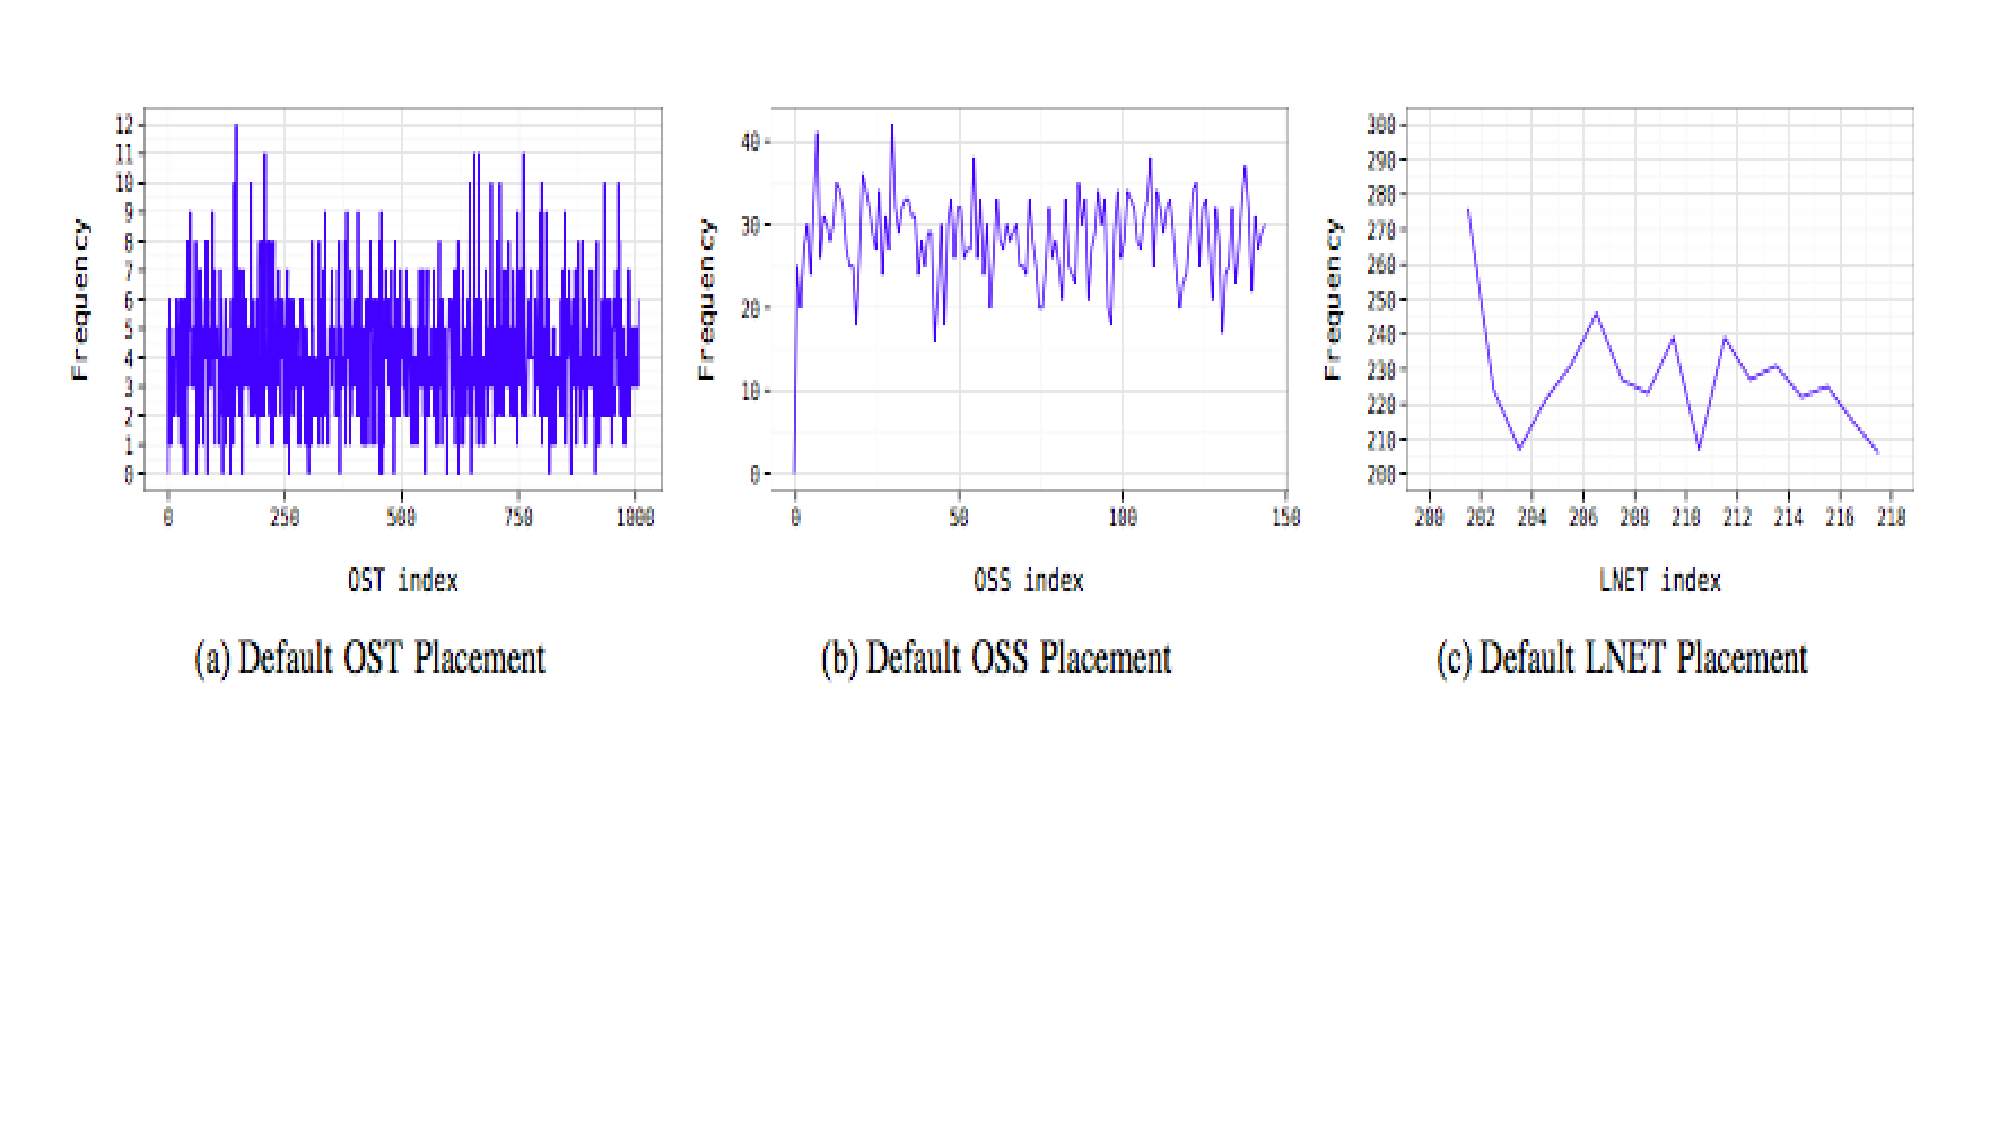
\includegraphics[width=\columnwidth]{graphics/infrastructure.pdf}\vspace{-1.2in}
  \caption{Resource usage distribution for OST(a), OSS(b) and LNETs(c). }
\end{figure}


% This is about finding the relationshiop of workload-dependent to workload-independent metrics. -- Carlos
 %are driven from multiple different approaches. First, supporting
%capability runs is a priority for capability machines. We propose to address
%capability run performance by incorporating monitoring for prepartory runs at
%smaller scale to profile the application output characteristics both from a
%writing velocity and volume, but also for example read patterns for the data
%analytics required to generate scientific insights from the raw data. 

% Not sure how to reuse this ... -- Carlos
%By
%discovering approximate data proportions that will likely be the key subsets
%targeted by the simulation run, we can generate a policy to preserve a certain
%storage portion for high fidelity data storagae and use slower or perhaps lower
%fidelity or compressed data storage for less interesting data portions. We will
%support spreading data appropriately across the storage hierarchy. In
%particular, we will investigate how to place data across different layers to
%meet the performance requirements for output while maintaining system
%availability for other applications and offering the best possible performance
%for the data analytics that will ultimately process this data.


% Not sure how to reuse this... -- Carlos
%Second, once data has been placed for future performance requirements, policies
%must be able to address maintaining data on a priority basis in that location
%to deliver on the placement optimization generated by the capability run
%profilier.

% This is a matter of metering, not performance reservations. -- Carlos
%Third, most future NVM devices have limited write endurance prompting
%management to ensure fair use by all machine users. Technologies like
%NAND-flash and Phase Change Memory have limited write endurance. By
%incorporating policies about the proportion of write endurance a compute
%allocation is entitled to, data placement decisions can be made to ensure fair
%resource usage. While the offending application will suffer worse IO
%performance, other applications that more carefully address their data
%intensity on these limited devices will achieve higher overall performnce. Only
%by instituting such policies can we encourage application users to adopt
%technology to manage the limited resources.


%We propose to investigate both offering a policy mechanism and how to implement
%these kinds of policies in a way that addresses offering the shortest
%end-to-end time for scientific insights.


``Quality of Service'' (QoS) refers to the
properties of the performance qualtiy of a particular service, in
this case the storage system.
Performance quality can be expressed in either relative or absolute
terms. Examples of relative performance terms are ``fair'',
``proportional'', or ``priority/class-based'' (``the higher the
priority the better the service'' or ``1st class is better than
2nd''). The key advantage of relative performance terms is that
they are easy to implement. The key disadvantage is the difficulty
of making any guarantees based on those implementations --
even relative guarantees are mired by the well-known effect of
priority inversion~\cite{lampson:cacm80}. Examples of absolute
performance terms are ``rate-based'', ``soft real-time'', and
``hard real-time''. The key advantage of absolute performance
terms are that they enable the implementation of strong
guarantees: absolute terms enable agreements between application
tasks and storage that we call \emph{reservations} and that do not
change meaning depending
on the storage system's workload. The key challenge of absolute
performance terms is that their implementation is non-trivial,
especially in large-scale systems.

\paragraph{Approach:} The goals of this proposal require applications
to demand guarantees in terms of absolute performance qualities.
The first key enabler for any service to make absolute guarantees
is \emph{performance isolation}, i.e. the ability to shield the
performance impact of one task from another. The most straight-forward
but least flexible strategy is to simply cap the latency of each
task, irregardless of its completeness (see for
example~\cite{decandia:sosp07}). This strategy is applicable when
incomplete tasks still have value and missing results are either
not important or can be easily retrieved in subsequent tasks. A
more generally applicable strategy is to control the admission of
tasks to the system: \emph{admission control} maintains a
\emph{utilization model} that can predict the utilization of system
resources given a new task, estimates the current utilization of
the system, and decides whether the task can be admitted without
overloading the system. Thus, admission control avoids system
overload conditions that lead to hard-to-model chaotic behaviors.
Consequently, utilization models can frequently be approximated by
automatically calibrated linear models (see for
example~\cite{skourtis:hpdc12}).

Another essential component of performance isolation is the
\emph{charging model} which determines which task(s) should be
charged how much for a request. Performance isolation is implemented
by the charging model by ensuring that performance of a task only
depends on its reservation and its workload behavior (but not on
other workloads in the system). Each task has a budget based on its
reservation and spends it based on the cost of each request determined
by the charging model. A charging model determines the cost based
on the utilization model and the interactions a request can have
with other requests (e.g. a random request to spinning media
interrupting a stream of sequential requests).

Performance isolation (including its utilization and charging models)
critically depends on \emph{workload-independent metrics}. Even
though throughput and latency are frequently the most meaningful
metrics for an application, they are not workload-independent and
therefore are inadequate for measuring the utilization of a device
across all workloads, unless one accepts worst-case estimates that
can lead to gross underutilization of resources (e.g. the throughput
of random and sequential workloads in spinning media differ by
orders of magnitudes). A common workload-independent metric is
\emph{time utilization}, i.e. the amount of time a resource is
utilized in a given time interval. Time utilization has the advantage
of having an always defined maximum and therefore makes resources
fully reservable. Even though a workload-independent metric might
at first not appear meaningful for an application, given a particular
workload an application can discover the relationship between its
workload-dependent metric and the workload-independent metric.
Because of performance isolation, the application has to discover
this relationship only once.

\paragraph{Related Work:}

\paragraph{Challenges:} The deep and heterogenous memory and storage
hierarchy we are assuming for this proposal complicates the
relationship between workload-dependent and workload-independent
metrics: the performance of a task can significantly differ depending
on what levels of the hierarchy are involved. Furthermore, an
important goal of the proposed project is to enable applications
to reason about the trade-off between resolution and latency, adding
yet another dimension to how tasks are mapped to resources.

\begin{itemize}

\item A key challenge of admission control is scalability: the
decision of whether to admit a task could potentially depend on
global knowledge of the current utilization of every single resource
in the system. Scalability therefore depends on whether admission
control is able to accurately map a new task to a relatively small
set of resources which can quickly provide up-to-date utilization.
One approach might involve pseudo-random mapping that also load-balances
as a side-effect.

\item To offer latency/latency trade-offs, the system must be able
to quickly generate a number of data production plans, involving
different parts of the hierarchy and different data resolutions.
It will then use the utilization model to estimate the latency for
each production plan and the resolutions they can provide. Here
again, pseudo-random selection could reduce the number of resources
that would be involved, thereby increasing scalability.

\item The complexity of a utilization model involving the entire
storage hieararchy with 100,000s of devices is potentially daunting.
However, the utilization model can be simplified by modeling classes
of devices as well as classes of requests. In particular, each
device could restrict access to its content via a set of well-defined
methods with known, absolute performance properties.

\item Flash devices become inherently unpredictable when reads and
writes are mixed on the same device because of garbage collection.
While write latency can be easily hidden using asynchronous I/O,
hiding read latency is more difficult. By separating reads and
writes for each device, read latency becomes predictable. The
challenge is to minimize duplication of data, at least on fast
layers and leverage redundancy across layers.

\end{itemize}


%%% Local Variables:
%%% mode: latex
%%% TeX-master: "../proposal"
%%% End:


\subsubsection{Discovery}

%
% This has been merged into the Naming Servie subsubsection
%

Hierarchical Storage Management (HSM) systems offer a strct caching approach
for managing different storage capacities trading off performance for capacity.
By maintaining a single namespace across all tiers, it is possible to list a
single directory view with files stored at different tiers. While this approach
to managing multi-tier storage works, it is far from ideal for scientific
simulations.

Our goal with this proposal is to offer a similar capability, but use a finer
granularity. Instead of a single file such as might be used to store an entire
timestep output for a simulation, we will demonstrate offering the same
capability at a subset of a single variable level. By shifting to a
finer-grained approach, we will enable more effective use of close/fast/small
storage tiers. Traiditional HSM stores an entire file on a tier making room if
insufficient space is available. With this shift to a partial variable
granularity, a 1 PB output with 500 GB of ``high interest'' data can limit this
costly tier ussage to just 500 GB greatly enhancing usability.

Tagging a variable subset as ``high interest'' requires intervention from the
application and/or middleware to determine what data meets this criteria. The
storage system itself simply needs to offer an ability to perform different
actions based on this information.

The challenge for discovery is that potentially, data will migrate from where
it is initially stored to a new location within the storage system. Sirocco
offers an ability to search for data that has moved as well as forcing a
particular resilience-based replica be the ``authoritative'' version. We will
investigate if the current Sirocco functionality is capable of supporting the
new operating modes we wish to offer. Initial expectations suggest having
bounded time guarantees for finding data are critical for offering the quality
of service guarantees we wish to offer. This new work will be an expansion of
Sirocco's currently planned features.

The other aspect of discovery is the negotiation between the user and the
storage system for a data quality/retrevial time trade-off. The naming service
will work hand-in-hand with the discovery, data migration, and time estimation
services to offer the best possible options for data retrevial based on quality
of service requested.

\subsubsection{Eviction Metrics}

% The title might have to change...

There is a spectrum of approaches on how to leverage a memory and storage hierarchy: On one end of the spectrum is to copy or move data from one tier to another, the closer the tier to the hierarchy's top, the faster the access to the data it contains. On the other end of the spectrum is to use higher tiers exclusively for auxiliary data that to some extent represents the actual data on the lowest tier. Examples of auxiliary data are views, indices, lossy compressions, lower resolution data, and summary data (sometimes also known as metadata). There are a number of drivers that push 
\subsection{Naming and Discovery Service}
\label{sec:naming-discovery}
\paragraph{Background:}
Given the well documented difficulties with POSIX-compliant naming and our
approach that decomposes what would be a single file into potentially large
number of objects, we must take a new approach to naming.  Data migration, as a
result of system pressures or user/system policies, further adds to the
complexity of managing naming and discovery. Our naming service must maintain
sufficient metadata information, track or be able to find objects as they move
across storage layers, and facilitates data discovery. Since we need to also
support access through POSIX APIs for existing application and system
integration, we must address how to bridge the drastic differences between the
decomposed objects of potentially varying fidelity with potentially multiple
versions with a POSIX API-compatible interface.

Hierarchical Storage Management (HSM) systems~\cite{blaze:1992:hsm} offer a
strict caching approach for managing different storage capacities trading off
performance for capacity.  By maintaining a single namespace across all tiers,
it is possible to list a single directory view with files stored at different
tiers. While this approach to managing multi-tier storage works for whole files
that fit on single logical devices, it is far from ideal for scientific
simulations.

The overriding theme for this proposal of providing a cooperative relationship
between the user and the storage system extends into this area as well.
Negotiating the data quality/retrieval time trade-off requires additional
metadata.  Providing this functionality requires the naming service be able to
both return a list of data versions and an indication of data quality. This
will be combined with a retrieval time estimate for each version by the
middleware to determine what data version should be retrieved.  This estimate
will be discussed elsewhere in this proposal.

In addition to the basic naming and data tracking operations, we will also need
to incorporate authorization capabilities. Sirocco currently integrates with a
Kerberos service for authentication. Given a capability ticket, a user can
access different objects as needed. This ticket structure offers protection
services typically offered on POSIX directories and files, but can do it at the
fork level instead. This allows a reduced quality data version to be available
for the general users while the high-quality version would be limited to the
data creator. This and other considerations for security must be incorporated
into the entire naming and metadata service.

While strongly encouraging data to stay in a particular type of storage tier,
ultimately it must be possible to flush this data to make room for other uses.
Sirocco offers a ``flush'' operation that forcibly migrates data to the
long-term resilience requirements, freeing space in the scarce resources. In
many, if not most cases, this will move data towards or actually on to a device
like tape, intended for long-term storage.

\paragraph{Approach:}
Our goal with this proposal is to offer a similar capability but with a finer
granularity leveraging the inner structure of scientific data. It must also
handle data discovery efficiently for cases where data is spread across several
storage layers or some of those pieces may have migrated based on system
pressures or user or system policies. Instead of a single file, such as might
be used to store an entire timestep output for a simulation, we will
demonstrate a metadata service with naming at the science variable level, but
with an associated list of all of the variable pieces and potentially different
versions stored throughout the storage system. By shifting to a finer-grained
approach, we will enable more effective use of close/fast/small storage tiers
and prioritize objects with high importance.  Traditional HSM stores an entire
file on a tier making room if insufficient space is available.  With this shift
to a partial variable granularity, a 1 PB output with 500 GB of ``high
interest'' data can limit this costly tier usage to just 500 GB, greatly
improving storage availability in the close/fast/small tier and focus
performance/capacity costs to get the most science from the platform.  By
only placing ``high interest'' data in the close/fast/small tier, we will
effectively reduce pressure forcing data migration hurting both writing
performance and the later data analytics required for generating scientific
insights.  Sirocco identifies a data segment using a
container/object/fork/address tuple that can have associated attributes. We will
add both a special attribute indicating that this record is of ``high
interest'' as well adapting a migration mechanisms to use this attribute, if
present, to strongly encourage keeping the record in  the highest storage tier as possible. 

Meanwhile, we need to be able to locate or ``discover'' the data should it
move.  The challenge for discovery is that potentially, data will migrate from
where it is initially stored to a new location within the storage system.
Sirocco offers an ability to search for data that has moved as well as forcing
a particular resilience-based replica be the ``authoritative'' version
migrating the data to a particular location. We will investigate if the current
Sirocco functionality is capable of supporting the new operating modes we wish
to offer. Initial expectations suggest having bounded time guarantees for
finding data are critical for offering the quality of service guarantees we
wish to offer. Some potential approaches can build on CRUSH~\cite{weil:ceph}
from Ceph to offer a map of where to search for data sequentially. Given our
multiple storage tiers, we would extend this using some mechanism to shift to
the next tier to continue searching because the requested data never made it to
this location. This new work will be an expansion of Sirocco's currently
planned features.

We plan to address scalability problems by continuing with the LWFS and Sirocco
model. LWFS and Sirocco have taken an approach similar to the pure object
stores, but with a focus on the HPC setting. They have abandoned a fully POSIX
compliant metadata service as the default model in favor of a
container/object/fork/address tuple for identifying data similar to those used
for pure object stores. By having a service that addresses the object
collections that comprise a single thing, such as a variable or timestep
output, just enough metadata is maintained to make the storage system usable
without additional heavy lifting by clients.  LWFS demonstrated a POSIX-style
namespace on the side kept in sync using a transaction process like
D2T~\cite{lofstead:2012:txn} showing that this alternative approach can support
traditional POSIX API calls even though the underlying storage system uses a
different model. Because we are not requiring the entire storage space be
addressible from a single tree root, we can offer multiple independent roots
using the Sirocco object storage. We will investigate how to make the naming
and discovery service scalable under the circumstances outlined above.

\paragraph{Related Work:}
Structurally, the traditional POSIX naming service offering a hierarchical
space consisting of directories and files may be maintained for backwards
compatibility. However, this view will not offer the same strict semantics
POSIX defines. We must break these strict semantics to address scalability
problems forced by the serialized access to a single source for creating and
accessing files.  Several efforts~\cite{patil:2007:giga+,carns:pvfs} have
worked to reduce this contention by doing things like reducing the serialized
scope to a single directory or subtree, or allowing a single process in a
collective file operation talk with the metadata service and distribute a
handle to other participants. While these approaches help, they do not address
this key scalability limitation of serialized access--even if the metadata
service is spread across multiple nodes. Instead, we will offer a short
duration to consistency POSIX view to offer the performance and consistency
requirements an exascale application demands.

While pure object stores, such as those popular in the big data
domain~\cite{Fitzpatrick:2004:memcached}, others avoid this bottleneck by
strictly offering an object ID with the application required to manage how this
ID maps to something of interest. This approach of removing the metadata
service from the system level completely can work well for scale out
applications where data is created or consumed by a single process at a time or
just in a work queue rather than potentially O(1 million) processes all
actively collectively for a single ``object''. To address this case, having
some system integrated metadata services to associate names with these object
is a preferable solution. While it will not have the same synchronous
consistency semantics as POSIX, we will offer something as close as possible to
address legacy application and command-line style data access and migration to
other storage types using these POSIX semantics.

\paragraph{Challenge:}
The main challenge of incorporating the additional, rich metadata will be
joined by the additional challenge of coordinating with the other storage and
application-layer services to offer the best access times possible for data
stored in the system. The developed metadata services that drive data
compression and subsetting operations must have easy, consistent, and ideally
non-blocking or locking access to this metadata service. We must investigate
how to build such a metadata and naming service that also incorporates and
maintains the additional metadata required to support our advanced
functionality.

Our research in this area will address the following questions:
(1) Since our metadata is distributed and partitioned, how do we respond to user
  requests within a specified time bound with accuracy? How do we estimate the
  completeness of the response?, 
(2) For POSIX API requests, how do we respond if only varying data fidelity
  levels are available for the requested data object?, 
(3) What level of metadata should we maintain and keep in sync to enhance
  response quality within time-bound requests?, 
(4) How much time should be allowed for searching for metadata given the user
  specified limits for data retrieval since the user will still have to spend
  the data retrieval time from different devices? How do we integrate the read
  time overhead into the metadata requests?, and
(5) How do we provide appropriate security while maintaining scalability,
  particularly with the distributed metadata stores?

\begin{tightEnumerate}

\item {\bf Milestone 1}: Demonstrate a metadata service capable of serving both POSIX
clients and our clients, but without consideration for authentication,
authorization, or data migration.

\item {\bf Milestone 2}: Demonstrate a time bounded search approach for finding data
within the storage system to identify data and the current location.  This will
update the cached information in the metadata service to short-circuit future
requests for the data presuming that it does not migrate again soon.

\item {\bf Milestone 3:} Demonstrate incorporating {\color{red}A\&A (what does this stand for CHECK-tsr)} and show scalability under
both application load as well as storage system pressures, showing that we can
tolerate both loads and maintain quality of service.

\end{tightEnumerate}


\subsubsection{Estimation of Times}

Feiyi

There are two fundamental causes that can impede the I/O performance in an extreme-scale SSIO system. One is indirection, where layers of storage tiers are employed either for performance and/or for scalability reasons.  The direct consequence is that there could be multiple traversing paths from application end to the rest place of data, and more often than not, the I/O paths are not under control under any single authority. The other cause is the shared use of resources. The best effort I/O request/response nature and lack of QoS mechanisms imply that there is little guarantee in terms of expected performance.  Both indirection and shared use of resource contribute to a high probability of imbalanced use of resources thus the occurrence of congestion and degraded performance. Traditionally, there is a disconnection between storage infrastructure and rest of system software and applications: the infrastructure details are not exposed anywhere at all. One argument favoring this is to ensure a platform agnostic design. 

As an example to demonstrate that this disconnection will hurt system performance: We launch 4096 processes with each process doing a single file I/O operation against half of the Spider II file system. The traces of those files are analyzed to examine the utilization distribution of different components. Figure (a), (b) and (c) shows the resource usage distribution for OSTs, OSSes, and LNETs, respectively. We observe that there exists a significant variation in usage across components of any given type (e.g., OST, OSS or LNET). For example, some OSTs are used more than 10 times while some others are never used (corresponding to zero frequency count). Similarly, OSSes and LNETs show significant imbalance in usage under the default placement strategy. Consequently, imbalanced resource utilization increases the contention at certain components more than others. 

Given these insights, we advocate the idea that the infrastructure knowledge should find a way to relay to the upper layer for better and more effective use of resources.   We think this is more pertinent and critical given the recent development of multi-tier storage and storage component heterogeneity.  There needs to be a way for application/middleware layer to gain more exposure of storage system for more intelligent processing logic.  One prime example of such exposed knowledge can be request/response time. To most applications, this is a black box. Profiling it at the upper layer is neither efficient nor effective, as it doesn't reflect cross-layer characteristics. However, Most of storage layer does keep a detailed profiling of such information. We therefore envision and propose a histogram-based request/response profiling API that application and middleware layer can leverage and make more informative decisions.

\begin{figure}[tbh]
  \centering
  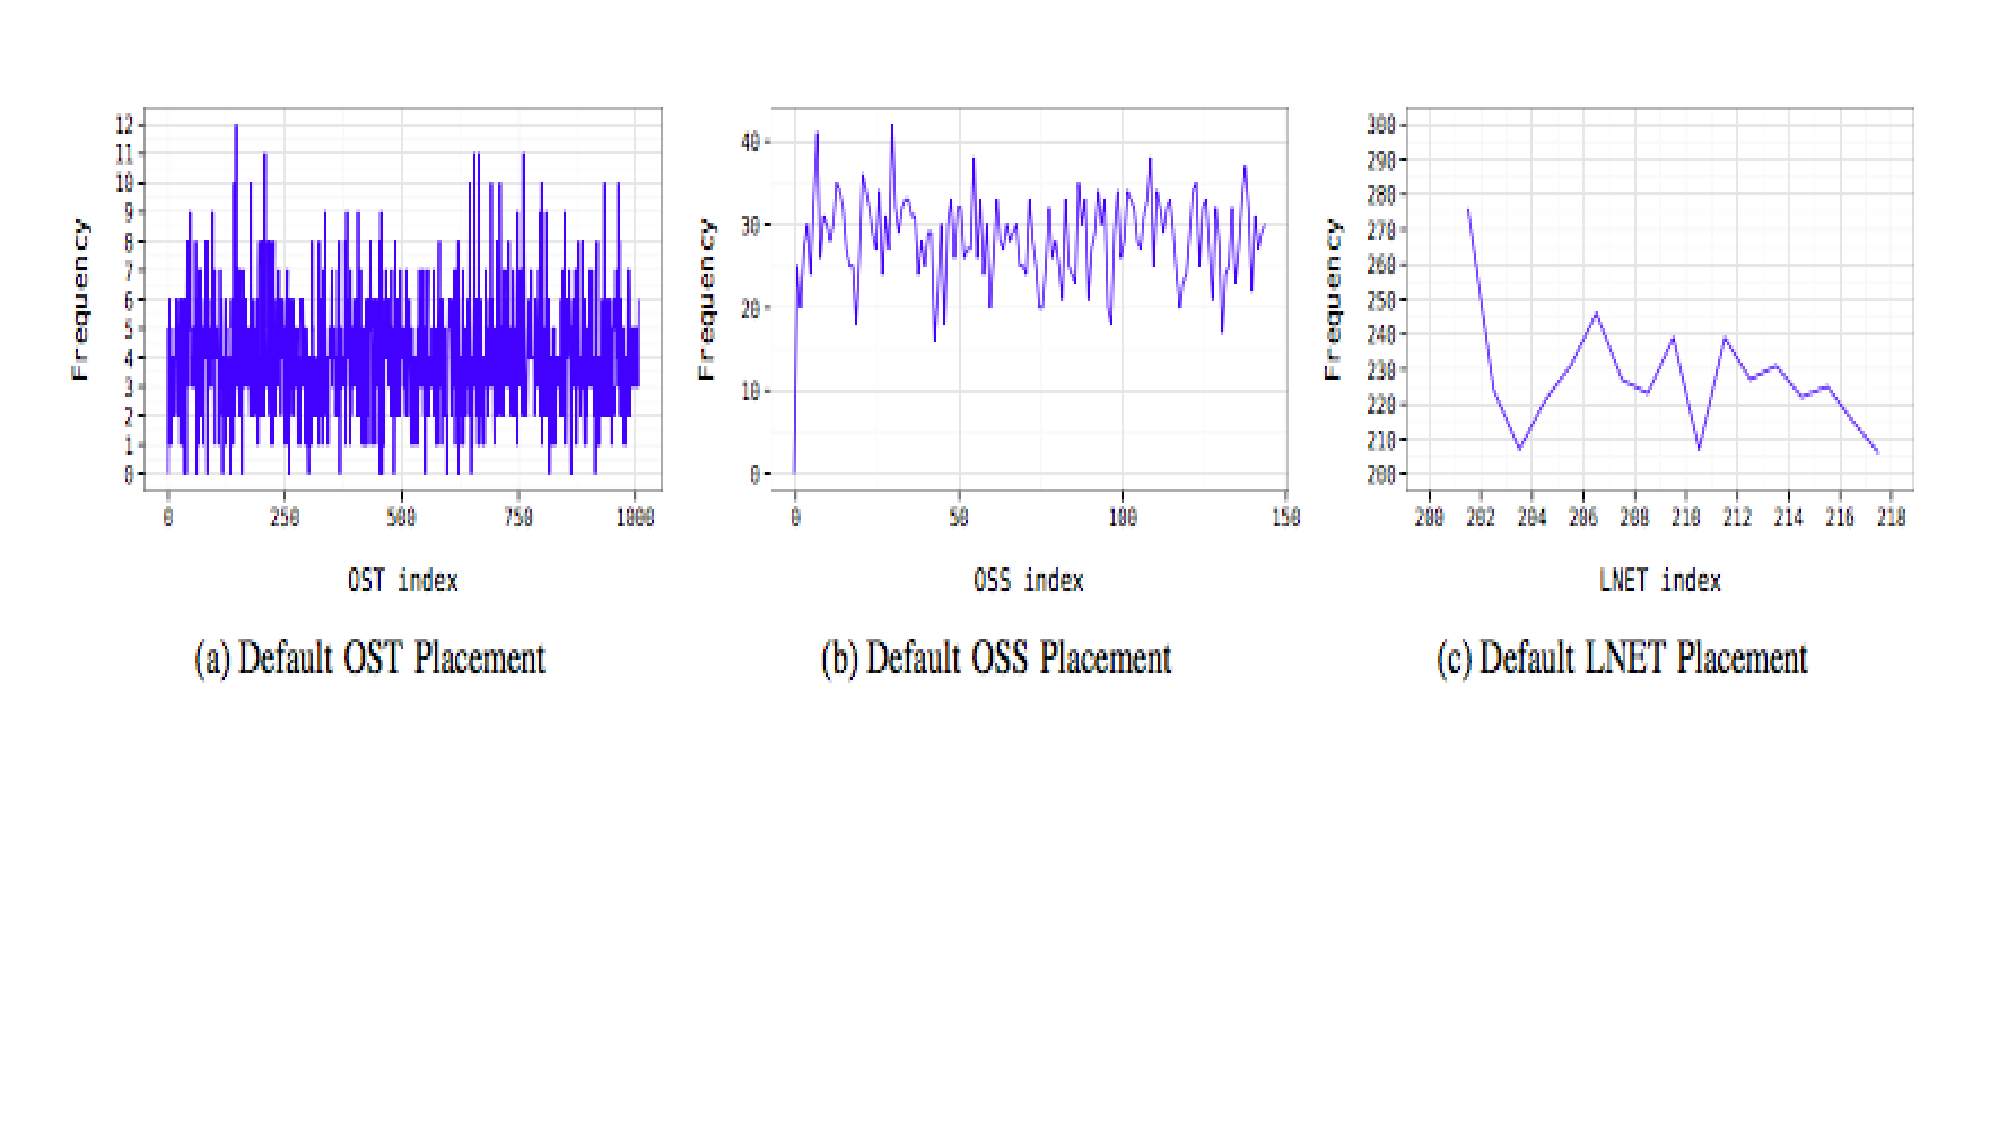
\includegraphics[width=\columnwidth]{graphics/infrastructure.pdf}\vspace{-1.2in}
  \caption{Resource usage distribution for OST(a), OSS(b) and LNETs(c). }
\end{figure}

%%% Local Variables:
%%% mode: latex
%%% TeX-master: "../proposal"
%%% End:



%%% Local Variables:
%%% mode: latex
%%% TeX-master: "../proposal"
%%% End:

\section{Deliverables}
The following are the per year project deliverables:
\small
\textbf{Year 1}
\begin{tightItemize}
\item Develop new techniques for data description that allow users to 
describe the data utility based on their expectations. (ORNL)

\item Assemble and evaluate general techniques for refactoring of data
that will be embedded in the system and can be selected by users or applications. (Brown/ORNL)
\item Explore the use of application hints and utility of data to guide the initial placement of data. 
(Rutgers/ ORNL)
\item Investigate the trade-off between ``filing'' and ``piling'' data. 
Demonstrate a time bounded search approach for finding data within the storage system
to identify data and the current location. (UCSC/ Sandia)
\item Demonstrate a metadata service capable of serving both POSIX clients and our clients. (Sandia/UCSC)
\end{tightItemize}

\textbf{Year 2}
\begin{tightItemize}
\item Develop a new type of querying system that allows an application to ask the storage system
about completion timing information. (ORNL)
\item Evaluate the effectiveness and overhead to re-organize data and use the multi-layer approach 
to staging. (Brown/ORNL)
\item Research autonomic data management strategies that
can evaluate utility/cost trade-off, and appropriately place/move data objects at runtime. 
Research runtime tracking and estimation. (Rutgers/ORNL)
\item Extend Sirocco to enforce data-centric metrics that help guide the QoS decisions. (Sandia)
(Sandia/UCSC)
\end{tightItemize}
\textbf{Year 3}
\begin{tightItemize}
\item Work with DOE applications, particularly XGC1, GTC, and SPECFM3D, to assess 
the new I/O interface including both APIs and hints. (ORNL)
\item Research techniques that can enhance migration without making the eventual 
lookup of data unbounded, and manage each tier in a scalable fashion. (ORNL)
\item Demonstrate incorporating A\&A and show scalability under both application load as
well as storage system pressures showing that we can tolerate both loads and maintain quality of
service. (Sandia)
%\item storage APIs to manipulate storing and retrieving data to specific tiers
%\item metadata management for data stored in multiple tiers using different compression
%\item metadata management for deeper data knowledge
%\item middleware hooks to manage new storage APIs
%\item example lossy and lossless compression plug-ins to demonstrate the effectiveness of this approach
\end{tightItemize}
\normalsize

\section{Management}
\label{sec:management}

Careful management will be required to ensure that the problems and delays that are inevitable in any research project
do not unduly disrupt overall progress. To this end, we define a detailed workplan,
establish a  management structure with defined oversight responsibilities, and establish a schedule of regular meetings and
reviews to ensure progress.  We will use google docs to share documents, emails lists for informal communications and a 
weekly phone call in the main research areas to discuss project tasks and milestones. 

Dr. Klasky will oversee the outcome of this project,  Dr. Abbasi (ORNL) will lead the Application Interface area, and Dr. Lofstead
will lead the Storage System. This project is focused on the tight integration of application aware-middleware and a storage system backend.
Our team has a strong track record of tight-collaboration, with both Drs. Abbasi and Lofstead both working with Dr. Klasky for their Ph.D. at the Georgia
Institute of Technology.  Our structure includes an area lead for each major research area plus
an integration lead responsible for coordinating periodic integration tests. The area leads plus the project PIs
form the management team, which will meet weekly to review progress and revise plans as needed.
We will also have a {\bf Science Advisory Board} consisting of one application Scientist, Dr. C. S. Chang (PPPL), one storage system expert from the 
OLCF, Dr. Vazhkudai (ORNL) who we will advice us yearly on our project goals and outcomes and make adjustments accordingly. We will also have our
lead Math Lead, Dr. Ainsworth, to work with the applied mathematics community to ensure that the hierarchical decomposition of data will work in theory
for current and next generation exascale simulations. 

We will conduct six-monthly {\bf integration tests}  to validate our ability to combine models, apply
combined models to real problems, and cope with the challenges of real data. We apply this approach routinely
in other projects and find that it helps to focus effort and identify problems early. The tasks of defining,
scheduling, and running critical post hoc reviews of integration tests will be coordinated by the Integration Lead, Dr. Parashar. 
These meetings will bring all hands together at least once a year.

We will monitor and report {\bf success metrics} including: 
research publications;
our ability to predict and explain performance of I/O workloads on the current machines., in different environments;
our ability to reduce data and characterize data from an object into multiple bins, 
our ability to integrate our routines into the Sirocco file system and test the feasibily on current and next generation LCF systems, and
how tools lead to workflow performance improvements, for both reading and writing data from our exemplar applications which we will test.

\section*{Summary}

We will do good stuff because it must or we won't get any good science done ever
again.

}{
\section{Introduction} 
\label{sec:introduction}

{\em The purpose of computing is insight, not numbers}~\cite{Hamming:book}.
Richard Hamming's remark, made over 50 years ago at the dawning of the age of
large scale scientific computation, is even more relevant today as we prepare
for scientific simulation at exascale. 
The central objective of this proposal, ``minimizing the time knowledge" from 
scientific computing, aligns perfectly with this sentiment. 
%Hamming was a pioneer in the fields of coding theory, scientific computing and 
%information theory who would instantly sympathize with the central objective of 
%this proposal--minimizing the time to knowledge.  

Avoiding impending bottlenecks in exascale scientific discovery will require
new research into managing and storing the large amounts of data that will be
produced by simulations and analyzed for months afterwards.
%
In this project we will demonstrate a cooperative approach for storing data
where the user and the storage system work together to achieve the best
possible utility and performance given data features, storage tier
characteristics, and current system state. We will investigate novel techniques
to facilitate efficient mapping of data objects, even partitioning individual
variables, from the user space onto multiple storage tiers and enable
application-guided data reductions/transformations to address capacity and
bandwidth bottlenecks, while constraining errors to be within user provided
bounds.
% 

We will address the associated I/O and storage challenges in the context of
current and emerging storage landscapes and expedite insights into critical
scientific processes, while demonstrating the validity of our approach in key
DOE domains. We will research techniques for creating and using a Scalable 
Storage Software Infrastructure, and integrating services from the middleware 
layer with Storage System capabilities to support novel strategies for distributing 
data both horizontally and vertically across the storage system.  Negotiation between
these layers will be provided as a fundamental service, allowing users to
easily save ``the best'' amount of data, which is automatically placed throughout the
entire storage stack.

The metric we are most interested in optimizing is time to knowledge.  Current
approaches to addressing the I/O bottleneck fall into two broad categories:
parallel file system approaches that optimize the throughput for an entire
system, and I/O middleware approaches that optimize the performance of a single
application. Both approaches have been successful to date, but are unlikely to
overcome the remaining obstacles in reaching exascale. 
Instead of trying to optimize throughput, we will seek to reduce the time to knowledge. 
This is the most significant metric for scientific applications where the desired outcome
is not storing data, but rather executing a knowledge creation and extraction processes 
on the data. 
Moreover, we aim to perform the optimization not for a single
application, but rather for workloads within a multi-user multi-application
system environment.

Our approach targets the expected characteristics of exascale storage hardware.
The storage layer will be partitioned into multiple heterogeneous tiers with
vastly different performance characteristics. The layers will be further
differentiated by the constraints on capacity and data lifetime within each
layer. Tape archival storage will still maintain data long term, but access to
this data will be orders of magnitude slower than the next layer and naively
accessing data from archival storage will greatly impact productivity.
%
Our approach in this proposal is to enable researchers to place more knowledge
into the SSIO system so that data can be recast from a sequence of bytes to
information, which the system can then place and optimize the time to gain
knowledge from exascale simulations.  We first motivate this by a problem our
team has been working on in the past six months, and then recast this problem
into a series of research questions and challenges which must be addressed in
order to optimize the SSIO system for exascale science.

The traditional approach to transforming results of scientific computation into
knowledge consists of storing the numerical output of a simulation on disk,
followed by a post-processing or analysis stage that might take place over
several ensuing weeks or months. Clearly, given the computation expected at the
exascale, this type of workflow is simply not viable.

%
\section{Scalable Storage Software Infrastructure}
Our focus in this proposal is in theme 2: Scalable Storage Software Infrastructure. We will focus on a state of the art
SSIO solution to solve problems which researchers are beginning to face and will make science on exascale systems
problematic without new insights and solutions.

Take for example the latest use case for the XGC1 simulation from C. S. Chang (PPPL), who is one of the largest users of Leadership Class Facilities (over 300M hours at ALCF, NERSC, and OLCF). They launched a series of simulations, planning to produce 100~PB of data over 10 days of total runtime on the Titan system. An expert team was assembled from the user group, the middleware I/O team to help with the application I/O (ADIOS), the local experts of the Lustre file-system and the tape archival system (HPSS). Due to physical resource limitations, the simulation was restricted to write about 10~PB initially. However, once the time to write and read, together with the financial cost to archive this much data were more fully explored, this plan was again signficantly reduced. At each stage, the particular expert knowledge regarding the lustre file system and the archival tape storage were not known to the user team. As these particulars were realized, significant modifications in the plans were made. Eventually, the user was forced to make very hard decisions in reducing the desired 100~PB over a 10-day run to a mere 5~PB of data. A maximum of 2~PB would be on disk, and the rest would be archived.

This forced the team to decide which pieces of data to save from the large amount of data; in 
other words, they had to prioritize which were the most important pieces and save only those. They had to further break down the still large data into two categories, data which they thought they would touch after one or two days of runs are completed and after the whole simulation is going to be completed (after ten days of runs), and what they would do with these different categories of data (the access pattern of the large data). 

They then had to develop new application specific data reduction techniques, and encode that into the application code itself on top of ADIOS, the middleware I/O layer. They then had to implement a crude discovery system to understand
which pieces of data were stored on the parallel file system and which pieces were on tape, and also which pieces were moved over to PPPL for immediate analysis by the user.

This solution worked well for the first day of run but after the second day more problems occurred: the variability in the time that it took to write the data made the I/O prohibitively expensive, because even though the project had reserved the majority of the resources at the OLCF, the file system was shared and sometimes the writing time took less 100 seconds, and at other times it was over 1,000 seconds. There was no method for the application or the user to monitor and predict this resource usage and to dynamically adapt to write less data when the I/O time was going to be longer. The greatest problem, however, comes after the simulation   completes: even to visualize the reduced data, just to get a first look at the visualization data, it could take over a month because some of the timesteps will be on tape and other timesteps will be on the file system. There is no method to just look at the data quickly at some level of quality quickly and understand which regions of the simulation to focus on in more detail.

The overarching idea of this proposal is that data from applications can be characterized by different
levels of importance and different levels of importance over time, which then can be used to guide the analysis and visualization later to access the most important data and deliver some level of knowledge without waiting for access to the whole original dataset. Information about the importance of the data at the application level, information about resource status and performance of the multi-level storage system, and flexible data reorganization and reduction operations at all levels can be utilized to provide a quality of service and allow users to gain insight in a timely manner.


To address these challenges we are proposing to combine knowledge
from a wide range of sources including ORNL applications, the ADIOS project,
the SNL Lightweight File Systems project and storage system knowledge, the metadata
management and storage systems knowledge of UCSC, and the middleware expertise
of Rutgers. We will integrate this diverse expertise to investigate how to make
a data, workflow, and application aware storage system.

%ADIOS was developed with the understanding that we must
%not only address the bottlenecks for current applications and
%hardware platforms but also provide a path forward for the next
%generation of applications and systems that would need to both
%maximize bandwidth to the storage system and also support
%transparently working around the storage system bandwidth
%limitations with new techniques and tools. To support the
%diverse operating modes of both using persistent storage and
%other data storage and processing technology, we made a
%great effort to provide a simplified interface to application
%developers, offering a simple, portable and scalable way for
%scientists to manage data that may need to be written, read
%or processed during simulation runs. This required abstracting
%away many decisions typically made in the application code
%so that they may be configured externally.
%In addition to this abstracted interface with external configuration
%options, common services were incorporated to afford
%optimizations beyond those for a single platform, such as
%buffering, aggregation, subfiling, and chunking with options
%to select each based on the data distribution characteristics
%of the application. A variety of asynchronous I/O techniques
%have been investigated and are being integrated with ADIOS.
%A recognition of application complexity has led to new techniques
%for testing I/O performance by extracting I/O patterns
%from applications and automatically generating benchmark
%codes. And finally, the march toward exascale has fueled the
%need to consider additional features such as compression and
%indexing to better cope with the expected tsunami of data.



We will examine the research challenges from the perspective of
%
(1) the user of the system who is attempting to run an exascale simulation,
%
(2) the Storage System and I/O layer which needs to negotiate between all of
the users, and finally
%
(3) the user of the system who is attempting to understand the data
produced by a set of simulations.

\subsection{Writing Perspective}
\label{subsec:sim-perspective}
The simulation scientist ideally should be able to
obtain an estimate of how much time will be required to write their data,
and how much storage space they will be able to get during the lifetime of
their simulations. Furthermore, they would like the ability to get an assurance
of Quality of Service such that they can react appropriately when the
expected bandwidth, for example, is less than what they desire. Ideally, the user
would specify a set of rules with which the system can make autonomic
decisions to determine what should be done.
%

One of the key aspects of our approach is to allow the users to define the
utility of their data; in other-words, the system should provide a
mechanism such that, for each data object, a user can specify pieces of the object
which have more utility (more importance).
There are many research challenges faced with
this approach including: 1) How do we make this simple enough so that users can
do this, 2) Can we define a model to allow the system to make
autonomic decisions to save the data which has the highest utility, and 3) Can
we allow the back-end storage system to interact with this model so that
it can optimize not just a single application but across all of the
applications.
 %
  In our simple scenario, a user wants to write 1~PB of data every hour
for checkpoint/restart, and they wish to write 500~TB of data every 15
minutes to save data for analysis and visualization. At this stage, they will ask the system to
write the data, and they would like to get an estimated time from which they can
then figure out, through a series of rules, whether they want to write out all
of the data, postpone the write until a later time, or write a reduced amount
of data using in situ reduction techniques, along with some code
container that allows for regenerating the data with a specified level of
accuracy.  Furthermore, they realize that the analysis data will be saved on
either the parallel file system, long-term tape storage, or on the campaign storage,
which is a medium-term storage
area with lower bandwidth than the parallel file system.
For each piece of data, the user will specify the lifetime so
that the data with the highest utility is kept around in fast storage for the longest
period of time, while the data with the least utility may be the first to be migrated to
lower layers of the storage hierarchy. 

Since the data will be a collection of objects placed on the storage system,
some of the objects will be broken up into multiple pieces by ``plug-ins''
to the system which will allow data to be characterized first in terms of the most
important pieces, and then by subsequent levels of detail. We can think of this as
something similar to an Adaptive Mesh Refinement scheme which keeps track of
the places where there are features such as steep gradients, which contain large errors on the
coarser views, as opposed to other areas with smaller errors. These distinctions allow us to make decisions
about which sub-objects to save (all of the data, which will then go to
different layers) or just some of the sub-objects? The research questions
are numerous: How does the user specify their intentions? How does the user
prioritize the different sub-objects of the data? Where does the data go
into the storage hierarchy? Does the data get replicated in the lower tiers
of the hierarchy? When the user specifies the time they want the data saved,
how does this get into the storage system?

\subsection{Storage System Perspective}
\label{subsec:storage-perspective}
From the perspective of the storage system, it is necessary to manage the data from
a given user request amongst all of the requests from all users, and try to optimize the
entire system accordingly. Today the problem is that when a user writes there is a
tremendous amount of interference from other users on the system who may be
writing or reading at the same time. By requiring a certain quality
of service the {\bf {\color {red} system must potentially lock out users with lower currency
they want to place in the reading or writing of their data}}. The storage
system must also automatically move data from one tier of the storage to
another, without affecting the quality of service that was offered at request
time. The storage system must be able to organize
data amongst all of the tiers of storage in a known, consistent way.

One of the main research objectives of this project is to understand how the
storage system can interact with the middleware (which is application-aware)  so
that the data with the highest utility is kept on the fastest layers of the
storage system for as long as specified. We need to maintain 
QoS and therefore, be able to provide fuzzy estimates of the time it will take to write/read data from
the different layers to inform any migration/eviction decisions, an it
is also critical that the storage system can manage (discover and retrieve) the data across all of the
layers automatically, without user intervention. We will use learning techniques to automatically migrate data
sub-objects across the hierarchy as well as to eventually evict data which is
large and has very low utility.


\subsection{Reading  Perspective}
\label{subsec:reading-perspective}
From the perspective of the users who want to read in the data from their
simulations, and then operate on this data and possibly write data, we see
that in general these users will be running on much less compute resources
than the users who are running the simulation. One of the important aspects
of this class of user is that they want a reduction of latency and they
require a certain amount of quality of service as well. When someone is
doing interactive analysis and expects that the data they read in is about
10s, but it turns into 1,000s, the user typically tends to either wait
another day for doing their analysis or gets frustrated and reads much less
data than they really need to. Furthermore the user tends to read in just a
small sample of the data without much knowledge if they are missing
important pieces of the data.

Our proposal will be responsive to theme 2 in the call, and we summarize them in the following table.
\begin{table}[htbp]
\vspace{2ex}
\begin{center}
\begin{tabular}{ | p {0.2cm} | p{5cm} | p{7.5cm} | p{1.6cm} |}\hline
\multicolumn{2}{|c|}{\bf Call area} & \multicolumn{1}{|c|}{\bf Relevant S2E2 work} & \multicolumn{1}{|c|}{\bf See} \\\hline\hline
%\multicolumn{2}{|c|}{Collaboration} & 
\multicolumn{2}{|p {5.5cm}|}{Approaches to improve the ability of SSIO software to support checkpoint/restart;} & 
General piece we are doing for this... & 
\S\ref{sec:?}, \S\ref{sec:??}, \\\hline
1 & Data abstractions & What will we do & \S\ref{sec:?}, \S\ref{sec:?}, \S\ref{sec:?} \\\hline
2 & Mapping science data models onto hierarchical storage & What we are doing & \S\ref{sec:?}, \S\ref{sec:?} \\\hline
3 & Mechanisms for data movement across the storage hierarchy & what are we doing. & \S\ref{sec:?} \\\hline
4 &  Extend the interaction of IO middleware with the resource management system & What we are doing & \S\ref{sec:?}, \S\ref{sec:?}  \\\hline
5 & Design and implement of IO middleware architectures  & What we are doing & \S\ref{sec:?}, \S\ref{sec:?}, \S\ref{sec:?} \\
\hline
\end{tabular}
\end{center}
\end{table}



%
%Exascale scientific discovery will be severely bottlenecked without
%sufficient new research into managing and storing the large amounts of data
%that will be produced during the simulation, and analyzed for months
%afterwards.
%%
%In this project we will demonstrate novel techniques to facilitate efficient
%mapping of data objects, even partitioning individual variables, from the
%user space onto multiple storage tiers, and enable application-guided data
%reductions/transformations to address capacity and bandwidth bottlenecks,
%while constraining the error to be within user provided bounds.
%%
%We will address the associated I/O and storage challenges in the context of
%current and emerging storage landscapes, and expedite insights into critical
%scientific processes, demonstrating the validity of our approach in key DOE
%domains. Our techniques will be to research novel techniques into a Scalable
%Storage Software Infrastructure by integrating services from the middle-ware
%layer which will talk to the applications, with the Storage system. The
%negotation between these layers will be a fundamental service which we will
%create in this project to ensure that users will be able to save `'the
%best'' amount of data in the different storage tiers.
%
%The metric we are most interested in optimizing is time to knowledge.
%Current approaches to addressing the I/O bottleneck fall into two broad
%categories. Parallel file system approaches that optimize the throughput for
%an entire system, and I/O middleware approaches that optimize the
%performance of a single application. Both approaches have seen success but
%are unlikely to overcome the major obstacles in reaching exascale. Instead
%of trying to optimize throughput, we will seek to reduce the time to
%knowledge. This is the most significant metric for scientific applications
%where the desired outcome is not storing data, but rather executing a
%knowledge extraction process on the data. Moreover, we aim to perform the
%optimization not for a single application, but rather for workload of a
%multi-user multi-application system environment.
%
%Our approach leverages the expected characteristics of exascale storage
%hardware. The storage layer will be partitioned into multiple heterogenous
%tiers with vastly different performance characteristics. This difference
%between layers will be further exacerbated by the constraints on capacity
%and data lifetime within a layer. Tape archival storage will still maintain
%data long term, but access to this data will be orders of magnitude slower
%than the next layer and naively accessing data from archival storage will
%greatly impact productivity.
%
%We will achieve reduced time to knowledge using a combination of techniques;
%\begin{enumerate}
%\item Data annotations specified at the application level to quantify the
%  relative important, utility and lifetime of data objects;
%\item Partitioning of data objects across the storage hierarchy utilizing
%  the additional knowledge embedded in the annotations;
%\item Evaluating the tradeoffs at runtime to guide data placement, movement,
%  and migration across storage layers using models, heuristics and
%  continuous learning;
%\item Utilize the additional knowledge available about the data to perform
%  application-aware data compression and I/O prioritization;
%\end{enumerate}
%
%We are aiming to spread an output across the vertical layers of the storage
%hierarchy simultaneously. When data should migrate to a higher tier, what
%happens to the existing version?
%
%Is there a canonical copy that is the originally written version?
%
%Is there annotation about this (I think so) attached to that part of the
%variable?
%
%At the tape layer, we see having a lossy compressed version just above the
%tape layer used as a directory/index and then the ``full'' resolution
%version on tape only retrieving once the user accepts the time/quality
%tradeoff. This is going to require some serious language to describe. If we
%have 100s PB of tape space, we'll need 1s PB of disk even at a 99\% data
%reduction. That is non-trivial.
%
%What happens when that data is retrieved from tape? Is a third copy made in
%an appropriately sized/quality level version for the tier it is requested to
%be pulled to? What if it is just the index version? Or the on tape version?
%Does it have a TTL because of the pain retrieving it from tape?
%
%Do we specify a target tier or just allow the system to place it in a place
%that makes sense? Given the potential space limitations, I think this is
%pretty critical because it could cause evictions or other insufficient space
%actions that are unintended. I can see us specifying that when you ask for
%data to be pulled at a particular quality level to a particular performance
%tier that it is a best effort with the use specifying if compromise or just
%failure is the result if the request cannot be fulfilled. Making this
%interaction make sense is going to require some reasonable thought and
%testing. We'll probably need to run it past apps people to get their
%feedback too as I don't think we are able to give a solid answer without
%some broad input.
%
%How does the migration to ``data lakes''/``campaign storage'' work? How does
%the migration to tape ultimately happen? I think we need to incorporate some
%explicit staging commands to move data both up and down the stack along with
%some variability in placement based on data features and current system
%state.
%
%Given the storage scarcity, particularly for NVM, I think we need to have a
%solid story here as part of the proposal. Yes, there are questions that have
%to be answered to build this still, but we need to have some pretty solid
%clarity where possible. I don't feel like I can explain it well enough at
%what I believe to be a proper clarity level at this point.

%%% Local Variables:
%%% mode: latex
%%% TeX-master: "../proposal"
%%% End:

}

% \input{narrative/ResilienceBigData3}
%% \input{narrative/timeline}
%% \section{Management}
\label{sec:management}

Careful management will be required to ensure that the problems and delays that are inevitable in any research project
do not unduly disrupt overall progress. To this end, we define a detailed workplan,
establish a  management structure with defined oversight responsibilities, and establish a schedule of regular meetings and
reviews to ensure progress.  We will use google docs to share documents, emails lists for informal communications and a 
weekly phone call in the main research areas to discuss project tasks and milestones. 

Dr. Klasky will oversee the outcome of this project,  Dr. Abbasi (ORNL) will lead the Application Interface area, and Dr. Lofstead
will lead the Storage System. This project is focused on the tight integration of application aware-middleware and a storage system backend.
Our team has a strong track record of tight-collaboration, with both Drs. Abbasi and Lofstead both working with Dr. Klasky for their Ph.D. at the Georgia
Institute of Technology.  Our structure includes an area lead for each major research area plus
an integration lead responsible for coordinating periodic integration tests. The area leads plus the project PIs
form the management team, which will meet weekly to review progress and revise plans as needed.
We will also have a {\bf Science Advisory Board} consisting of one application Scientist, Dr. C. S. Chang (PPPL), one storage system expert from the 
OLCF, Dr. Vazhkudai (ORNL) who we will advice us yearly on our project goals and outcomes and make adjustments accordingly. We will also have our
lead Math Lead, Dr. Ainsworth, to work with the applied mathematics community to ensure that the hierarchical decomposition of data will work in theory
for current and next generation exascale simulations. 

We will conduct six-monthly {\bf integration tests}  to validate our ability to combine models, apply
combined models to real problems, and cope with the challenges of real data. We apply this approach routinely
in other projects and find that it helps to focus effort and identify problems early. The tasks of defining,
scheduling, and running critical post hoc reviews of integration tests will be coordinated by the Integration Lead, Dr. Parashar. 
These meetings will bring all hands together at least once a year.

We will monitor and report {\bf success metrics} including: 
research publications;
our ability to predict and explain performance of I/O workloads on the current machines., in different environments;
our ability to reduce data and characterize data from an object into multiple bins, 
our ability to integrate our routines into the Sirocco file system and test the feasibily on current and next generation LCF systems, and
how tools lead to workflow performance improvements, for both reading and writing data from our exemplar applications which we will test.

%% \section*{Summary}

We will do good stuff because it must or we won't get any good science done ever
again.




\nottoggle{preproposal}{

%%%%% Bibliography %%%%%%%%%%%%%%%%%%%%%%%%%%%%%%%%%%%%%%%%%%%%%%%%%%%%%%%%%%%%

\renewcommand{\bibname}{ }
\bibliographystyle{cv}

% Multiple bib files are possible.  Format is comma separated list,
% relative to this directory, without .bib suffix.  So bib/a,bib/b,...


%------------------------------------------------------------------------------------------------------------------------------------------------------------------------
%%%%%  BIOSKETCHES
\clearpage
\phantomsection
\markboth{}{}
\addcontentsline{toc}{chapter}{Appendix 1. Biographical sketches}
\section*{Appendix 1: Biographical sketches}
% Generated by bin/config-personnel on Thu, Jul 09, 2015  4:55:08 PM

\chapter{Biographical Sketches}
\label{sec:bios}

\noindent
Biographical sketches of the senior personnel follow in alphabetical
order.  

\minitoc

\newpage

\smartinclude{Scott Klasky --- \ornl}{bios/klasky}
\newpage
\smartinclude{Hasan Abbasi --- \ornl}{bios/abbasi}
\newpage
\smartinclude{Gary Liu --- \ornl}{bios/liu}
\newpage
\smartinclude{Manish Parashar --- \ornl}{bios/parashar}
\newpage
\smartinclude{Gerald Lofstead --- \snl}{bios/lofstead}
\newpage
\smartinclude{Carlos Maltzahn --- \ucsc}{bios/maltzahn}
\newpage
\smartinclude{Lee Ward --- \snl}{bios/ward}
\newpage
\smartinclude{Kimmy Mu --- \ornl}{bios/mu}
\newpage
\smartinclude{Matthew Curry --- \snl}{bios/curry}
\newpage
\smartinclude{Feiyi Wang --- \ornl}{bios/wang}
\newpage



%

%%%%% 3.9 CURRENT AND PENDING SUPPORT
\clearpage
\addcontentsline{toc}{chapter}{Appendix 2. Current and pending support of the investigators}
\section*{Appendix 2: Current and pending support}
 \phantomsection
\vspace{2ex}
\noindent
Other support of the investigators follow in alphabetical order.
% Generated by bin/config-personnel on Fri Jan 17 21:40:41 EST 2014

\chapter{Other Support of Investigators}
\label{sec:other-support}

\noindent
Other support of the investigators follow in alphabetical
order.  

\minitoc

\newpage

\smartinclude{Hasan Abbasi --- \ornl}{other-support/abbasi}
\newpage
\smartinclude{Mark Ainsworth --- \gatech}{other-support/ainsworth}
\newpage
\smartinclude{Matthew Curry --- \oregon}{other-support/curry}
\newpage
\smartinclude{Scott Klasky --- \oregon}{other-support/klasky}
\newpage
\smartinclude{Qing Liu --- \oregon}{other-support/liu}
\newpage
\smartinclude{Gerald Lofstead --- \oregon}{other-support/lofstead}
\newpage
\smartinclude{Carlos Maltzahn --- \oregon}{other-support/maltzahn}
\newpage
\smartinclude{Kimmy Mu --- \oregon}{other-support/mu}
\newpage
\smartinclude{Manish Parashar --- \oregon}{other-support/parashar}
\newpage
\smartinclude{H. Lee Ward --- \oregon}{other-support/ward}
\newpage



%%%%% Bibliography %%%%%%%%%%%%%%%%%%%%%%%%%%%%%%%%%%%

\clearpage
\markboth{}{}
%\addtocounter{chapter}{1}
%\addcontentsline{toc}{chapter}{Literature Cited}
\addcontentsline{toc}{chapter}{Appendix 3. Literature cited}
\section*{Appendix 3: Literature Cited}
\phantomsection
\begingroup
\renewcommand{\chapter}[2]{}%
\bibliographystyle{abbrv}
\bibliography{bib/klasky,bib/abbasi,bib/maltzahn,bib/rutgers,bib/ainsworth,bib/liu,bib/lofstead}
\endgroup

%%%%% 3.10 FACILITIES %%%%%
\clearpage
\addcontentsline{toc}{chapter}{Appendix 4. Description of facilities and resources}
\section*{Appendix 4: Description of facilities and resources}
\phantomsection
% Generated by bin/config-institutions on Thu Jun 18 15:05:33 EDT 2015

\chapter{Description of Facilities and Resources}
\label{sec:facilities}

\noindent
Descriptions of institutional facilities and resources follow in
alphabetical order.

\minitoc

\newpage
\smartinclude{\ORNL}{facilities/ornl}
\newpage
\smartinclude{\SNL}{facilities/snl}
\newpage
\smartinclude{\UCI}{facilities/uci}
\newpage
\smartinclude{\BROWN}{facilities/brown}
\newpage
\smartinclude{\RUTGERS}{facilities/rutgers}


%%%%% DATA MANAGEMENT PLAN %%%%%
\clearpage
\markboth{}{}
\addcontentsline{toc}{chapter}{Appendix 5. Equipment}
\section*{Appendix 5: Equipment}

\vspace{2ex}
\noindent
ORNL has access to leading-edge computing platforms and services for the project through Oak Ridge Leadership Computing Facility (OLCF) as well as a mid-size cluster for data stream testing and workflow automation.
Our group at ORNL has access to a 40-node Opteron-based Infiniband cluster running Linux. The system is provided as an end-to-end resource for center users. It is used for workflow automation for jobs running from Titan and for advanced data analysis. The system contains 40 compute nodes. Each compute node contains four 2.3 GHz 8 core AMD Opteron processors, and 64 GB of memory. The system is configured with a 86 TB Lustre file system for scratch space, and has two SSD on each compute node.
The system is also connected to the center-wide spider system. In this proposal we will use the Lustre storage as ``campaign''
storage, and the SSD for testing our algorithms.

%%%%% DATA MANAGEMENT PLAN %%%%%
\clearpage
\markboth{}{}
\addcontentsline{toc}{chapter}{Appendix 6. Data management plan}

\phantomsection
\section*{Appendix 6: Data Management plan}

\vspace{1ex}
\noindent
The relevant data for the proposed work will be from the software we develop from our team, the documentation for our software, the performance data we use in our publications,
and the requirement documents we get from any of the users who we are working with.


Our team is  will be sharing these data artifacts with the broader community. ORNL will setup a dedicated website for this project which will have all relevant information, along with
a link to all of the new software that will be developed using an open source license.  The source code will be maintained using a versioning system and repository, Github, that is widely used and that we expect will also be well known for the next 10 years. 

The documentation will be made available online on the project web site. The performance data will be distributed through publications and technical reports. Publications and technical reports will be made available on the project web site as well. In addition, journal, conference, and workshop papers are also typically archived by publishers (e.g. ACM, IEEE, or Springer). Similarly, Oak Ridge and Sandia National Laboratories maintain archives of all the technical reports. The project web site will maintain pointers to all publications and reports, along with all data that was used in the publications.



%
%%
%\clearpage
%%\addtocounter{chapter}{1}
%%\addcontentsline{toc}{chapter}{Literature Cited}
%\addcontentsline{toc}{chapter}{Appendix 3. Literature cited }
%\phantomsection
%\bibliographystyle{abbrv}
%\bibliography{bib/klasky,bib/abbasi,bib/maltzahn,bib/rutgers,bib/ainsworth,bib/liu,bib/lofstead}
%
%
%%
%
%%%%%% Biographical Sketches %%%%%%%%%%%%%%%%%%%%%%%%%%%%%%%%%%%%%%%%%%%%%%%%%%%
%  %% Generated by bin/config-personnel on Thu, Jul 09, 2015  4:55:08 PM

\chapter{Biographical Sketches}
\label{sec:bios}

\noindent
Biographical sketches of the senior personnel follow in alphabetical
order.  

\minitoc

\newpage

\smartinclude{Scott Klasky --- \ornl}{bios/klasky}
\newpage
\smartinclude{Hasan Abbasi --- \ornl}{bios/abbasi}
\newpage
\smartinclude{Gary Liu --- \ornl}{bios/liu}
\newpage
\smartinclude{Manish Parashar --- \ornl}{bios/parashar}
\newpage
\smartinclude{Gerald Lofstead --- \snl}{bios/lofstead}
\newpage
\smartinclude{Carlos Maltzahn --- \ucsc}{bios/maltzahn}
\newpage
\smartinclude{Lee Ward --- \snl}{bios/ward}
\newpage
\smartinclude{Kimmy Mu --- \ornl}{bios/mu}
\newpage
\smartinclude{Matthew Curry --- \snl}{bios/curry}
\newpage
\smartinclude{Feiyi Wang --- \ornl}{bios/wang}
\newpage

%%
%%\section*{Appendix 2:Biographical sketches}
%%%%%% Other Support %%%%%%%%%%%%%%%%%%%%%%%%%%%%%%%%%%%%%%%%%%%%%%%%%%%%%%%%%%%
%
%% Generated by bin/config-personnel on Fri Jan 17 21:40:41 EST 2014

\chapter{Other Support of Investigators}
\label{sec:other-support}

\noindent
Other support of the investigators follow in alphabetical
order.  

\minitoc

\newpage

\smartinclude{Hasan Abbasi --- \ornl}{other-support/abbasi}
\newpage
\smartinclude{Mark Ainsworth --- \gatech}{other-support/ainsworth}
\newpage
\smartinclude{Matthew Curry --- \oregon}{other-support/curry}
\newpage
\smartinclude{Scott Klasky --- \oregon}{other-support/klasky}
\newpage
\smartinclude{Qing Liu --- \oregon}{other-support/liu}
\newpage
\smartinclude{Gerald Lofstead --- \oregon}{other-support/lofstead}
\newpage
\smartinclude{Carlos Maltzahn --- \oregon}{other-support/maltzahn}
\newpage
\smartinclude{Kimmy Mu --- \oregon}{other-support/mu}
\newpage
\smartinclude{Manish Parashar --- \oregon}{other-support/parashar}
\newpage
\smartinclude{H. Lee Ward --- \oregon}{other-support/ward}
\newpage

%
%
%%%%%% Facilities %%%%%%%%%%%%%%%%%%%%%%%%%%%%%%%%%%%%%%%%%%%%%%%%%%%%%%%%%%%%%%
%
%% Generated by bin/config-institutions on Thu Jun 18 15:05:33 EDT 2015

\chapter{Description of Facilities and Resources}
\label{sec:facilities}

\noindent
Descriptions of institutional facilities and resources follow in
alphabetical order.

\minitoc

\newpage
\smartinclude{\ORNL}{facilities/ornl}
\newpage
\smartinclude{\SNL}{facilities/snl}
\newpage
\smartinclude{\UCI}{facilities/uci}
\newpage
\smartinclude{\BROWN}{facilities/brown}
\newpage
\smartinclude{\RUTGERS}{facilities/rutgers}

%
%
%%%%%% Appendices %%%%%%%%%%%%%%%%%%%%%%%%%%%%%%%%%%%%%%%%%%%%%%%%%%%%%%%%%%%%%%
%%% \appendix
%%% \adjustmtc
%
%% Have we added the appendix line to the TOC?
%\provBoolDflt{addedappendixtoc}{false}
%
%\IfFileExists{appendices.tex}{ 
%  %% \phantomsection % Needed by hyperref because of the unnumbered section
%  %% \addcontentsline{toc}{chapter}{Appendices}
%  %% \setboolean{addedappendixtoc}{true}
%  \input{appendices} 
%}

% Normally only have this post-award
%% \ifthenelse{\boolean{includerevisedsow}}{
%%   \ifthenelse{\NOT\boolean{addedappendixtoc}}{
%%     \phantomsection % Needed by hyperref because of the unnumbered section
%%     \addcontentsline{toc}{chapter}{Appendices}
%%     \setboolean{addedappendixtoc}{true}
%%   }
%%   \input{revised-sow} 
%% }{}
}



\end{document}

%%% Local Variables:
%%% mode: latex
%%% TeX-master: t
%%% End:
\grid
